\documentclass[12pt]{article}
\usepackage{graphicx}
\usepackage{subcaption}
\usepackage[margin=1.0in]{geometry}
\setlength\parindent{0pt}
\usepackage[titletoc]{appendix}
\usepackage{float}

\bibliographystyle{unsrt}

\begin{document}

\title{Visualising Live Code Study Report - Draft 2}
\author{Arrian Purcell}

\maketitle

Two code visualisations have been analysed in a live coding context to determine effective presentational and educational features. Two visualisations were evaluated including a visualisation targeting aesthetic appeal and a visualisation with a more didactic approach. The goal was to determine the usability, differences and desirability of the two approaches to further inform future live coding visualisations.\\

The set of didactic visualisations predominantly focussed on the relationship between the live coding active processes and their behaviour. The visualisations prominently displaying the names of the active functions with visual indication of the number of functions running and their callback time. Bright colours and solid shapes were used to ensure constant visibility and communicate the intention of the underlying code. An example of this approach can be seen in Figure \ref{dvis}. Overall, four visualisations were presented with each introduced depending on the number of active functions. It was predicted that taking a more educational approach would see a reduction in audience confusion through the performance.\\

The set of aesthetic visualisations focussed less on the programmatic aspects of the live coding performance, rather intending to provide additional visual interest to the projected code thereby prolonging attention. More variety was used in visual structure and colour. An example of this approach can be seen in Figure \ref{avis}. Again, four visualisations were presented, varying the visualisation based on the number of active functions. It was predicted that focussing on the aesthetic nature of the visualisations would assist in audience retention and result in a consistency of interest through the performance.

\section{Method}

Two sets of visualisations were presented to an audience during a live coding performance and surveys were distributed. The performance was run as two ten minute improvised songs with each song demonstrating one of the two experimental visualisation conditions, either the didactic condition or the aesthetic condition. The experiment was run twice, with two separate participant groups, swapping the order in which the two sets of visualisations were presented to the audience.\\

The audience members completed a survey (see Appendix B) consisting of four sections over the course of the performance. These sections included a demographic information section, opinion of the first visualisation, opinion of the second visualisation and a section investigating the audience's overall opinion of the performance. The sections regarding the visualisations predominantly focussed on the enjoyment and understanding related to the visualisation while the final section focussed on eliciting potential improvements.\\

After explaining to the participants the structure of the experiment and allowing the participants to complete the initial demographic section of a survey, the live coder began the first performance utilising one of the two visualisations. Following this first set, the second section of the survey was conducted. A second set was then played using the alternative visualisation. Following this second set, the same survey questions were administered again, again asking the participants specifics about their enjoyment and understanding related to the specific visualisation demonstrated. A final survey question was then asked relating to their opinion regarding the whole performance and their suggested improvements.\\

To further inform the outcomes of the experiment a video-cued recall interview was conducted following the performance with the live coder. Two of the performances were examined critically and further discussion concerning the advantages and limitations of the visualisations were examined.

\section{Participants}

A total of 41 participants took part in the study. Over the two performances, 19 participants observed the first performance and 22 participants observed the second performance. The demographic makeup of the audiences was similar.\\

$66\%$ of the participants stated that they were male (see Figure \ref{genderdistribution}) and most participants were aged between 18 and 32 ($76\%$, see Figure \ref{agedistribution}). As the study was conducted within the Computer Science Department, a large proportion of the participants were experienced with programming with $90\%$ having current or previous experience with it (see Figure \ref{programmingdistribution}). Nevertheless, only $15\%$ of participants had previous experience with any of the Lisp style of languages (see Figure \ref{lispdistribution}), the style used within the performance.\\

Of the participants, $68\%$ stated that they listened to a large amount of music (see Figure \ref{musicdistribution}) though only about $15\%$ of participants stated that they played an instrument or sung regularly (see Figure \ref{instrumentdistribution}). Only $22\%$ of participants had seen a live coding performance before.

\section{Results}

Understanding and enjoyment were evaluated against the didactic and aesthetic visualisations. Results and statistical analysis of the differences between the aesthetic and didactic conditions follows. Note that for the following statistical analysis a significance level of $0.05$ was used with the chi-squared test for independence.

\subsection{Understanding}

Overall, $37\%$ participants stated specifically that the didactic visualisations helped them to understand the code, whereas $12\%$ participants stated that the aesthetic visualisations assisted in understanding the code.\\

$H_0$: There is no difference between the aesthetic visualisations and didactic visualisations in terms of understanding.\\
$H_1$: There is a difference between the two visualisations in terms of understanding.\\

A significant difference between the visualisations effect on understanding was found ($\chi^2=7.1986,df=2,p=0.02734$).

\subsection{Enjoyment}
Overall, for both visualisations, a large proportion ($> 50\%$) of the participants stated that the visualisations helped their enjoyment of the performance. Of the participants, $76\%$ stated that the aesthetic visualisations helped their enjoyment compared to $56\%$ participants that stated the didactic visualisations helped their enjoyment.\\

$H_0$: There is no difference between the aesthetic visualisations and didactic visualisations in terms of enjoyment.\\
$H_1$: There is a difference between the two visualisations in terms of enjoyment.\\

No significant difference between the two visualisations effect on enjoyment was found ($\chi^2=3.7733,df=2,p=0.1516$).

\subsection{Change in Understanding}

Participants were asked to rate their understanding during the beginning, middle and end of the performance.\\

During the didactic and aesthetic performances, $49\%$ and $44\%$ of the participants respectively stated that their understanding remained the same throughout the performance.\\

During the didactic performance, $10\%$ of the audience had an understanding that tended downwards (eg. high to low) compared to $20\%$ of the audience during the aesthetic performance meaning fewer audience members had a reduction in understanding through the didactic performance.\\

\subsection{Change in Enjoyment}

Participants were asked to rate their enjoyment during the beginning middle and end of the performance.\\

During the didactic performance, $15\%$ of the audience stated that enjoyment increased during the beginning remaining steady for the remainder whereas $24\%$ of the audience said the same during the aesthetic performance.\\

During the didactic performance, $22\%$ of the audience stated that their enjoyment decreased during the start of the performance whereas only $2\%$ stated the same for the aesthetic performance.\\

Approximately $30\%$ of the audience during both the aesthetic and didactic performances stated that their enjoyment remained steady throughout.\\

See Figure \ref{aestheticenjoymentchange} and Figure \ref{didacticenjoymentchange} for the distribution of changes to enjoyment between the aesthetic and didactic visualisations.\\

\begin{figure}[t]
\centering
\begin{subfigure}{.5\textwidth}
    \centering
    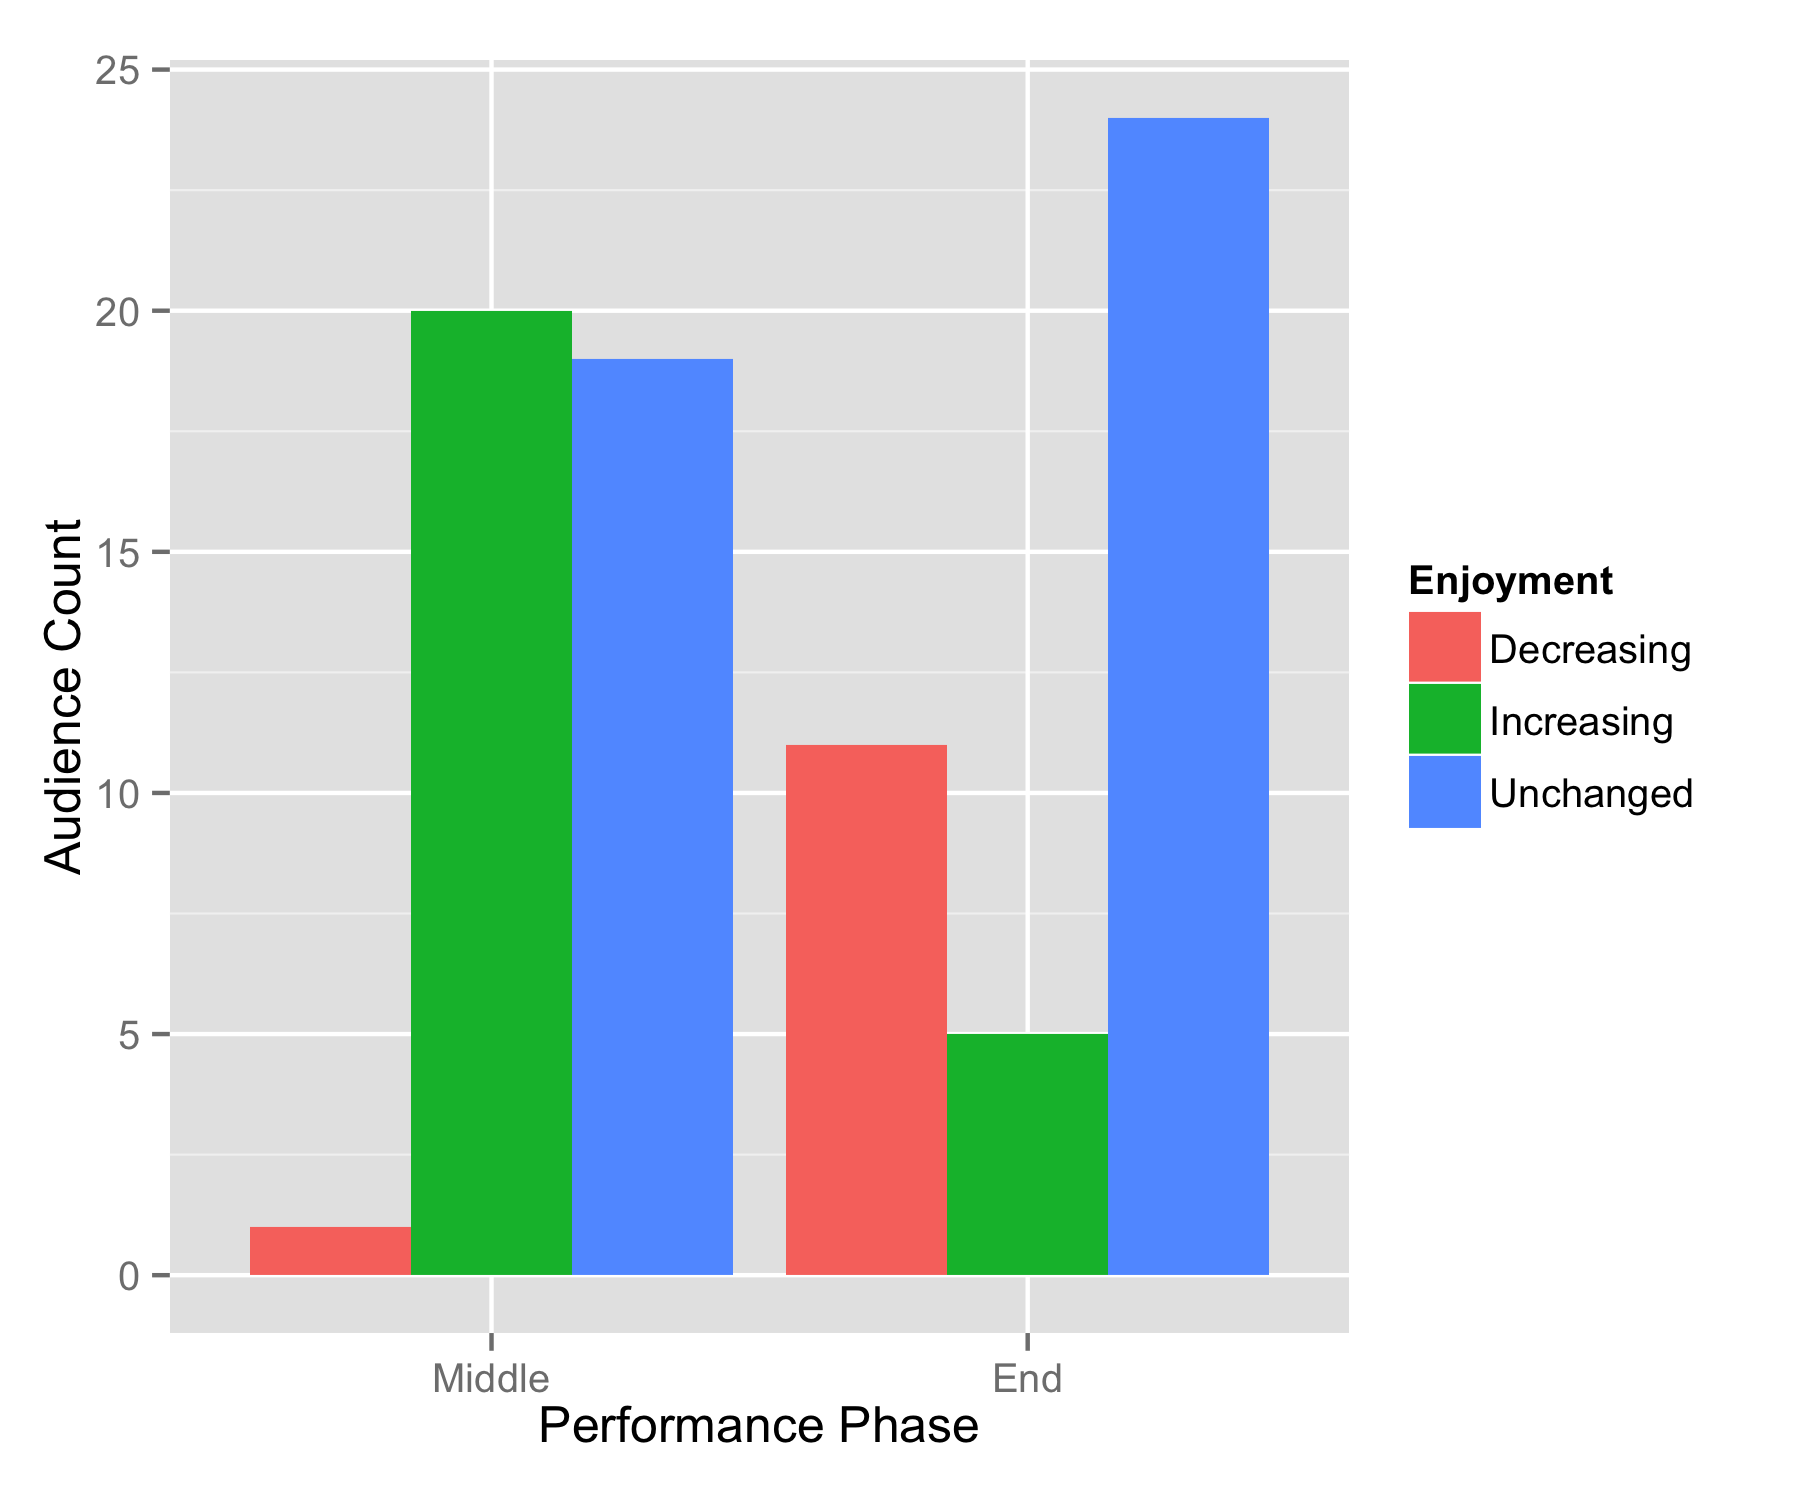
\includegraphics[width=1.0\linewidth]{graphs/enjoyment-change-aesthetic.png}
    \caption{Aesthetic Visualisation}
    \label{aestheticenjoymentchange}
\end{subfigure}%
\begin{subfigure}{.5\textwidth}
    \centering
    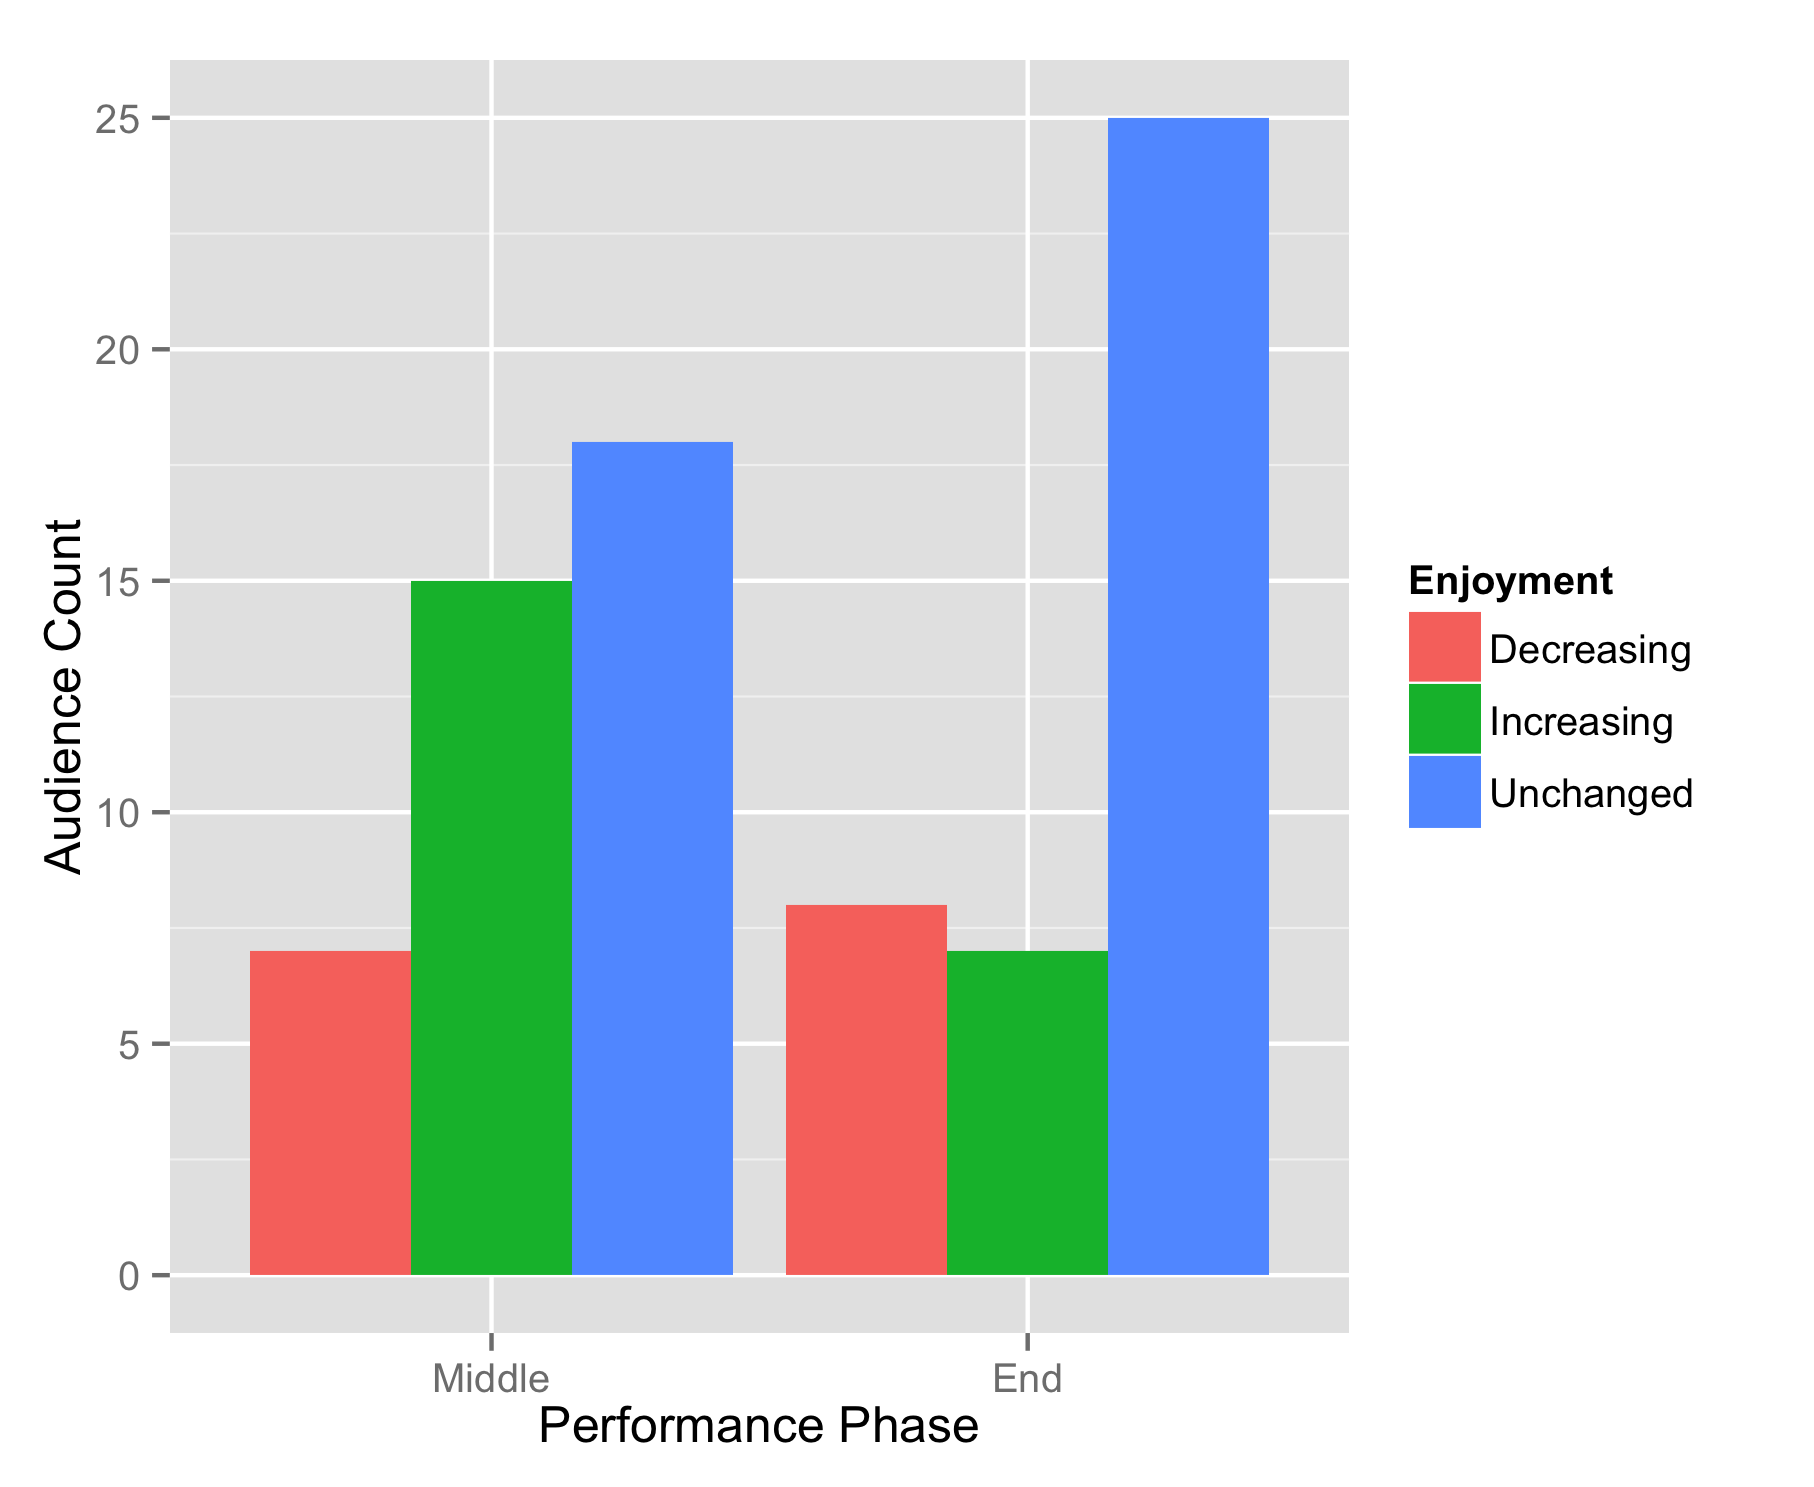
\includegraphics[width=1.0\linewidth]{graphs/enjoyment-change-didactic.png}
    \caption{Didactic Visualisation}
    \label{didacticenjoymentchange}
\end{subfigure}
\caption{Change of enjoyment through specific phases of the performance for aesthetic and didactic visualisations}
\end{figure}

\subsection{Liveness}

Participants were asked to discuss how each visualisation influenced or impacted the liveness of the performance. Concepts identified included positive and negative valence towards the didactic visualisations, positive and negative valence towards the aesthetic visualisations and the relevance of visual source code. 

within the discussion included the positive and negative aspects of the didactic visualisations, the positive and negative aspects of the aesthetic visualisations, source code discussion and statements indicating an understanding between the visuals and the source code.\\

Overall, $54\%$ of the audience indicated negative valence towards the didactic visualisation regarding liveness referencing a variety of reasons including that the ``visuals only responded to what was typed'', that the ``musical forms didn't occur at the most expected times'' and that the visualisations ``perhaps made the performance seem too polished''.\\

On the other hand, $34\%$ of the audience indicated positive valence towards the didactic visualisations suggesting that ``it was easier to follow this visualisation than the code'', ``the visualisations clearly showed the changes being made to the code'' and that these visualisations ``helped more with communicating that the performance was live''.\\

$40\%$ of the audience had negative valence towards the aesthetic visualisation its effect on the sense of liveness. Reasons cited include that the ``influence is not clear'' between the code and the visuals, that ``the visualisation did not make much sense'' and that the ``visualisations did nothing to suggest that the performance was live''.\\

$32\%$ had positive valence towards the aesthetic visualisation. A variety of the response included that these visuals were ``less dominating and more complementary'' and that ``the visualisations helped to show when a piece of code started working''.\\

A relatively large proportion ($28\%$) of the audience discussed the importance of the source code to the sense of liveness of the performance such as that the ``code showed what the musician was doing physically''. A further $5\%$ of the audience demonstrated a deeper understanding of the live coding process such as ``changing values produced changes in tone and speed of the music pitch''.\\

\subsection{Improvements}

The audience was asked to indicate possible improvements to the visualisations. 40\% of the audience suggested improvements that indicate a desire to see a better relationship between the visualisations and the music, with suggestions such as matching the visualisations to musical rhythms or pitch. For example, one audience member stated that the visualisations should ``perhaps have a stronger correlation with hush tones and defined shapes, baselines with wide and soft shapes with animations that follow the beat more consistently''.\\

Other members of the audience stated that they would like to see a better relationship between the code and the visuals. For example, one audience member stated that ``it would be really cool once you edit a code line and then activate it for it to morph into a visualisation for as long as this line of code is active''. Another audience member stated that ``it would be better to not just relate the function to the sound but relate every beat to the sound or to the code responsible for that beat''.\\

Other suggestions included increasing the readability of source code, increased immediacy of actions, increasing uniformity between the visualisations and the use of images to assist with the understanding of high level concepts.\\

\subsection{Follow-Up Interview}

A follow-up interview was conducted with the live coder to further examine the visualisation approach taken and the overall usability of the visualisations. See Appendix D for the full interview transcript.

\section{Discussion}

Overall enjoyment of the visualisations was high. This was the case for both the aesthetic and didactic visualisations.\\

The enjoyment of the aesthetic visualisation was higher and generally increased during the earlier stages of the performances suggesting that the aesthetic visualisations held the audience's attention consistently for a longer period (see Figure \ref{aestheticenjoymentchange}).\\

The didactic visualisation had a more constant decrease in enjoyment throughout the performance. Audience suggested improvements offer some insight with some stating that the visualisations were competing with the projected code. One audience member stated that they ``found them distracting'' and that they ``preferred just to read the code''. Given that more than half of the audience stated that both visualisations contributed positively to enjoyment, there is indication that the didactic visualisations contributed more to audience fatigue through the performance with decreased effectiveness during the later stages of the performances.\\

As expected, the didactic visualisations had a clear educational benefit over the aesthetic visualisations, contributing to increased understanding throughout the performance. Nevertheless, features of the visualisation still confused the audience. For example, one audience member stated that ``it felt harder to understand the code'' during the didactic performance than the aesthetic performance. Similarly, a number of audience members discussed the need for a better relationship between the visualisation and the music.\\

There was indication that the experience of the live coder and the experience of the audience was fundamentally different. For example, many members of the audience stated that they drifted between focussing on the music, focussing on the visualisations and focussing on the code. However, the live coder stated in the interview that his focus was dedicated purely to the code and the music rarely drifting. In one particular section of the interview, the live coder stated: ``I definitely wasn't paying attention to them on the day. In fact I tuned them out as best I can because I am just trying to focus on the code''. This conflicted with some members of the audience. For example, one stated that ``you could see the code being written and the visualisations helped to show when a piece of code started working''. \\

The strategy for audience members for either understanding or enjoying the performance proved to be different to that of the live coder. Regarding distractions, one audience member stated that ``the visualisations were interesting but distracting''. In comparison, when asked if the visualisations were distracting the live coder stated: ``Ah, no. In general I'm just so focussed on the code''. This difference may be due to the varying experience levels or the pressure of the situation.\\

\section{Conclusion}

An application of the visualisation of code to live coding has been examined. Results indicate the importance of providing visuals that complement the live coding performance. Visualisations targeted at the education of the audience showed a qualitative increase in understanding throughout the performance whereas visualisations targeted at the aesthetics of the music and performance indicated audience retention and a reduced fatigue effect over the didactic visualisations.\\

There was indication throughout audience feedback and the follow-up interview that the visualisations had potential. Desirable features within both visualisations could be further utilised building on the ideas developed including reacting instantly to code changes within the visualisations and providing a more effective visualisation of the relationship of code to music. These developments will provide a baseline for future visualisations.\\

One question to come from this study is the need to understand why the audience and the coder report such different experiences. Differences between the interview with the live coder and the audience feedback indicated a division between the goals of the audience and the coder.\\\\

\newpage
\section*{Appendix A - Survey Results}

\begin{figure}[H]
\centering
\begin{subfigure}{.5\textwidth}
    \centering
    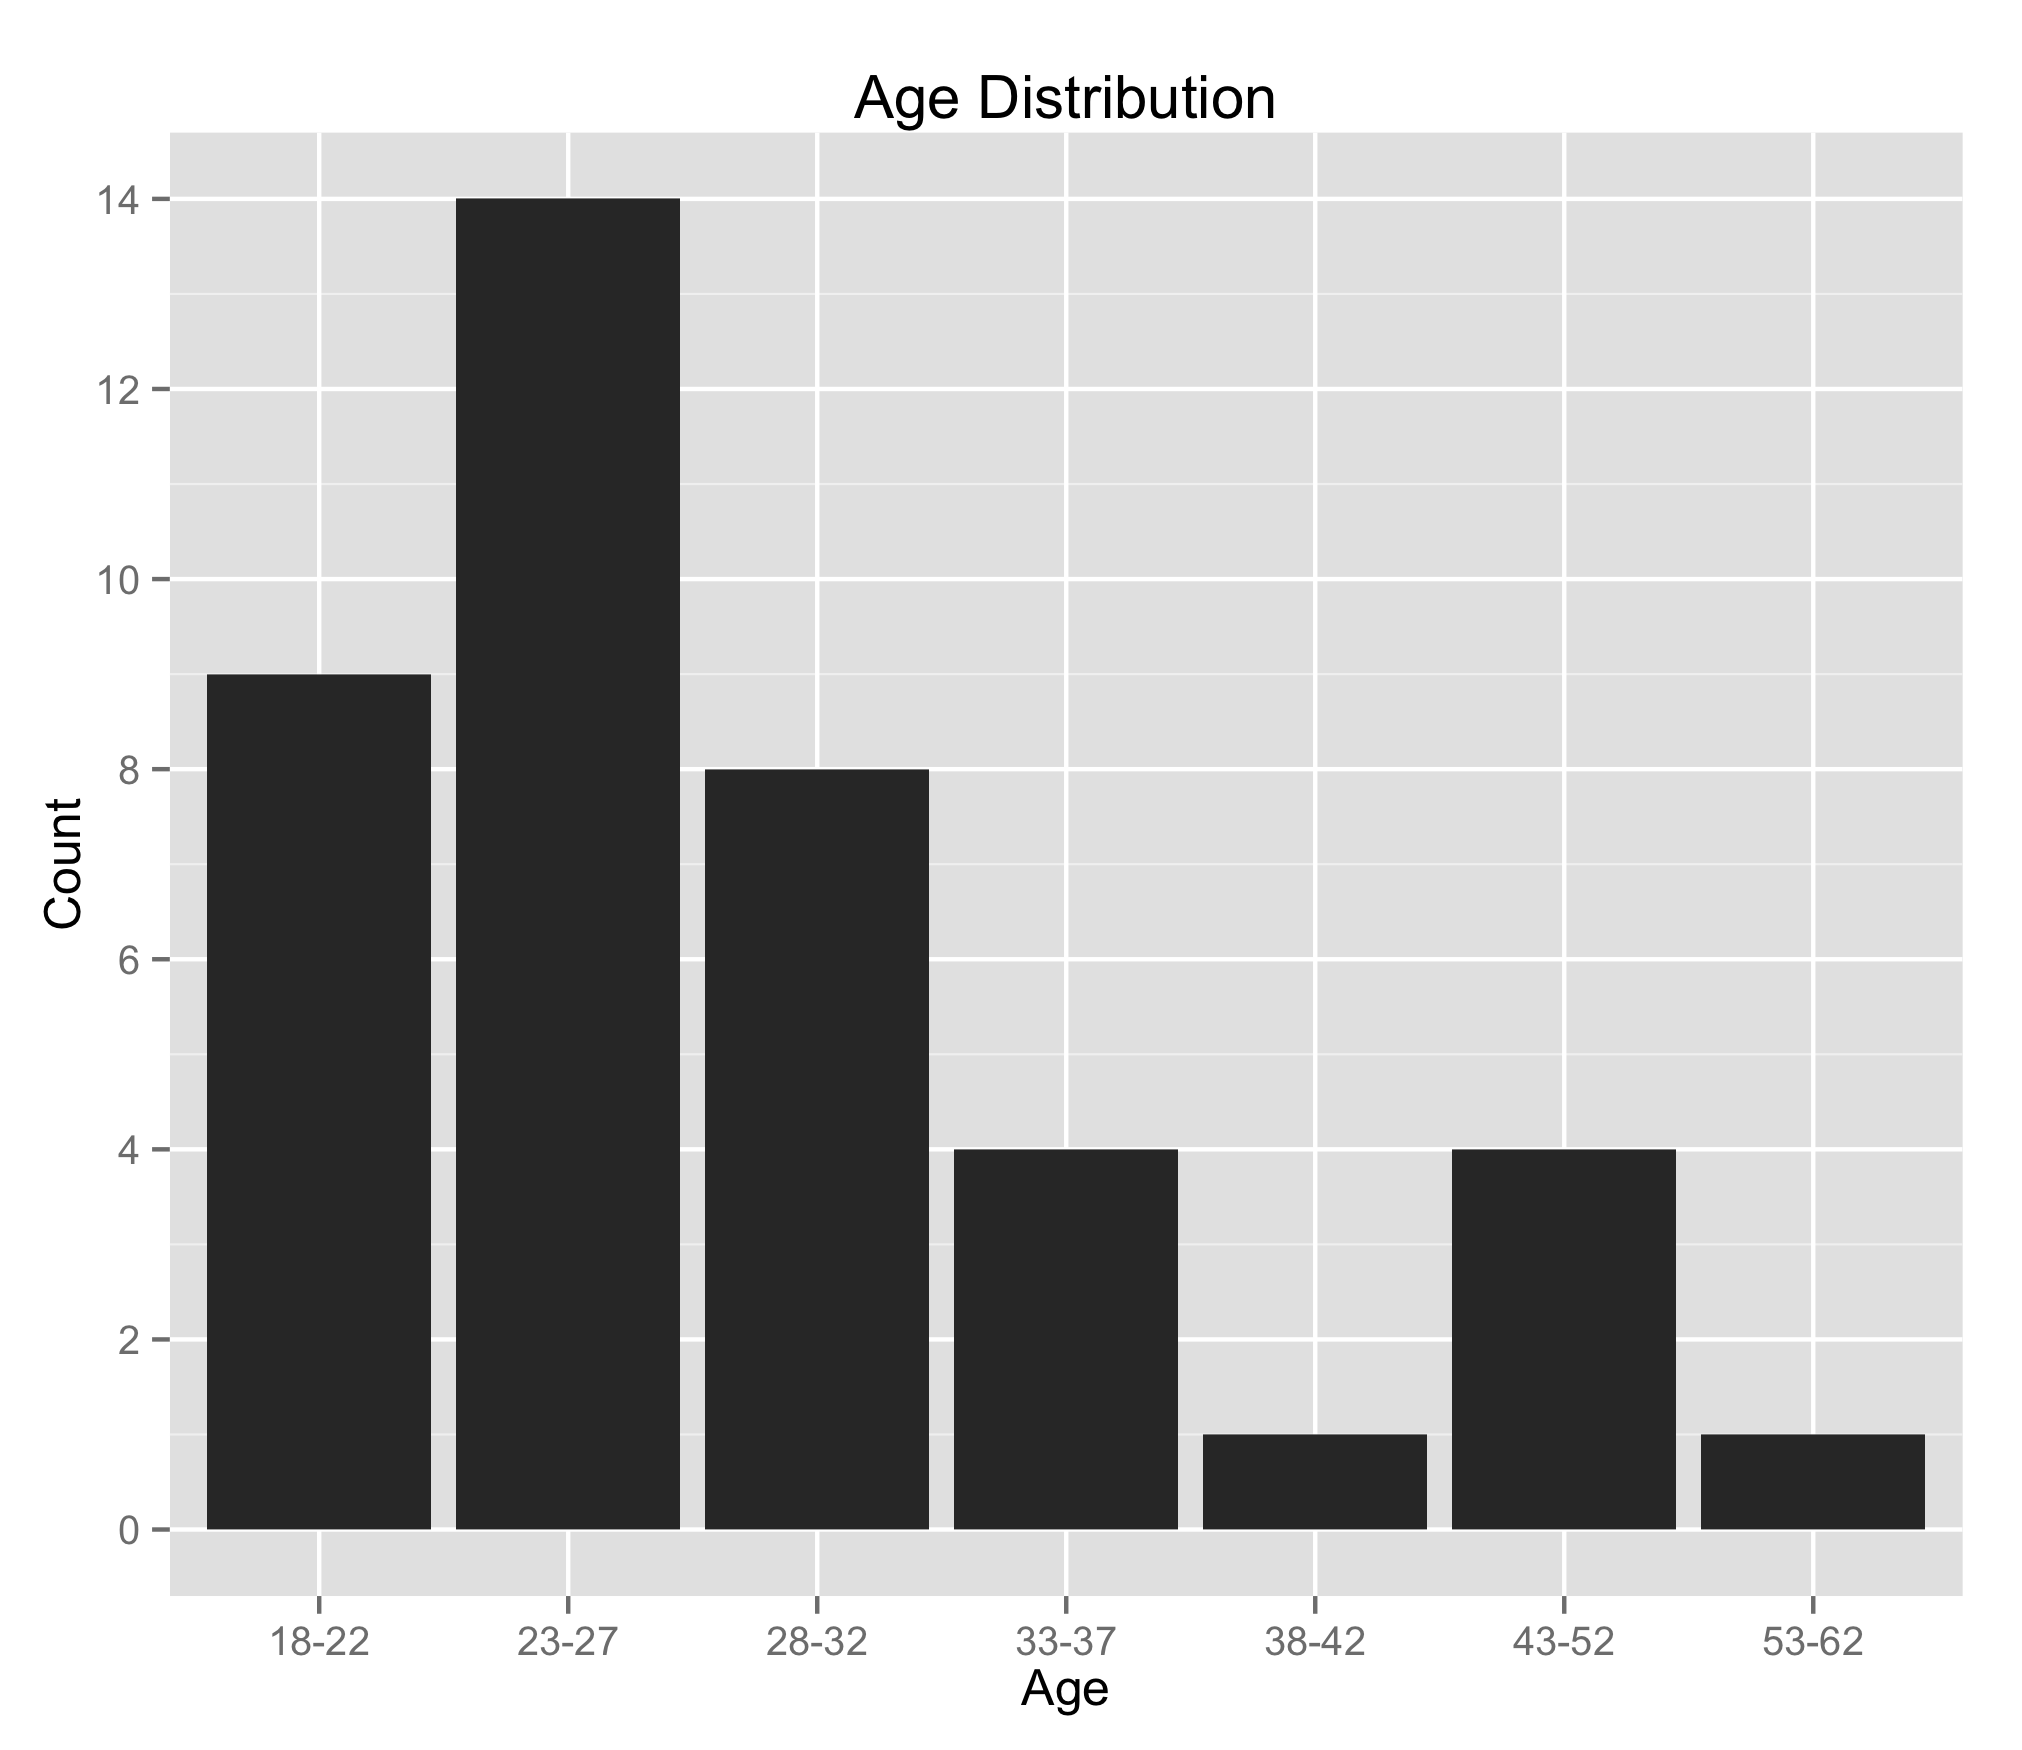
\includegraphics[width=1.0\linewidth]{graphs/age.png}
    \caption{Age Distribution}
    \label{agedistribution}
\end{subfigure}%
\begin{subfigure}{.5\textwidth}
    \centering
    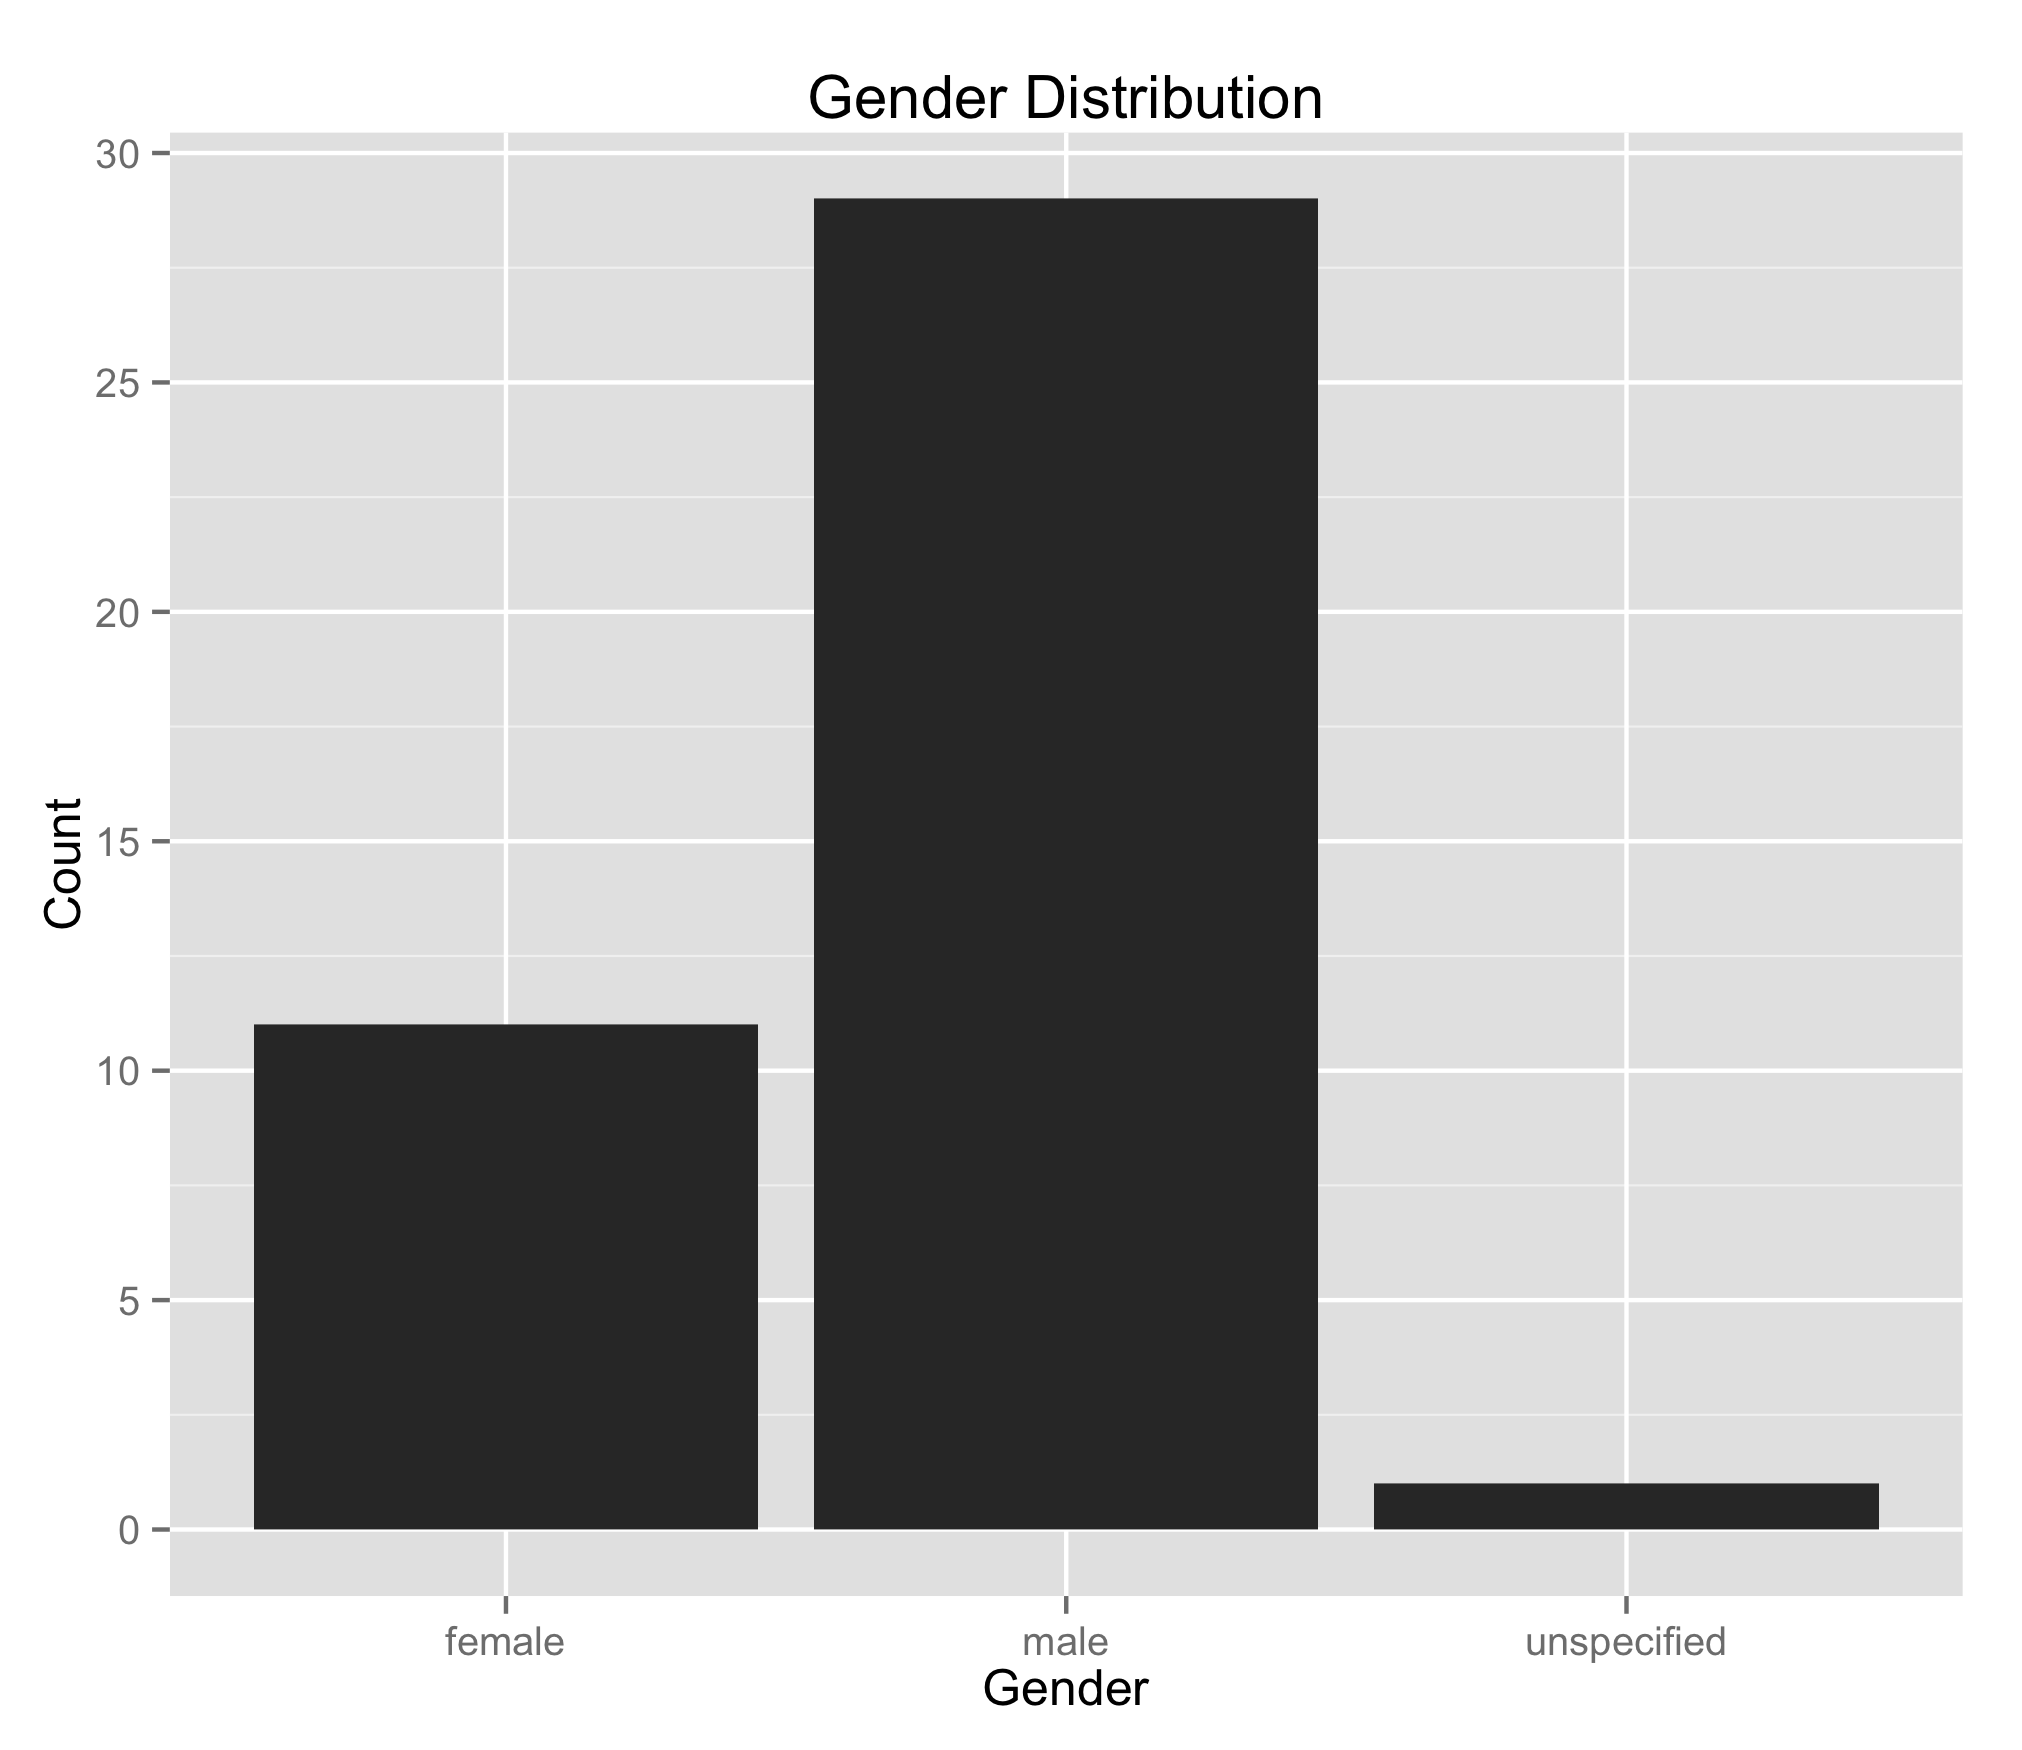
\includegraphics[width=1.0\linewidth]{graphs/gender.png}
    \caption{Gender Distribution}
    \label{genderdistribution}
\end{subfigure}
\caption{Basic Demographics}
\centering
\begin{subfigure}{.5\textwidth}
    \centering
    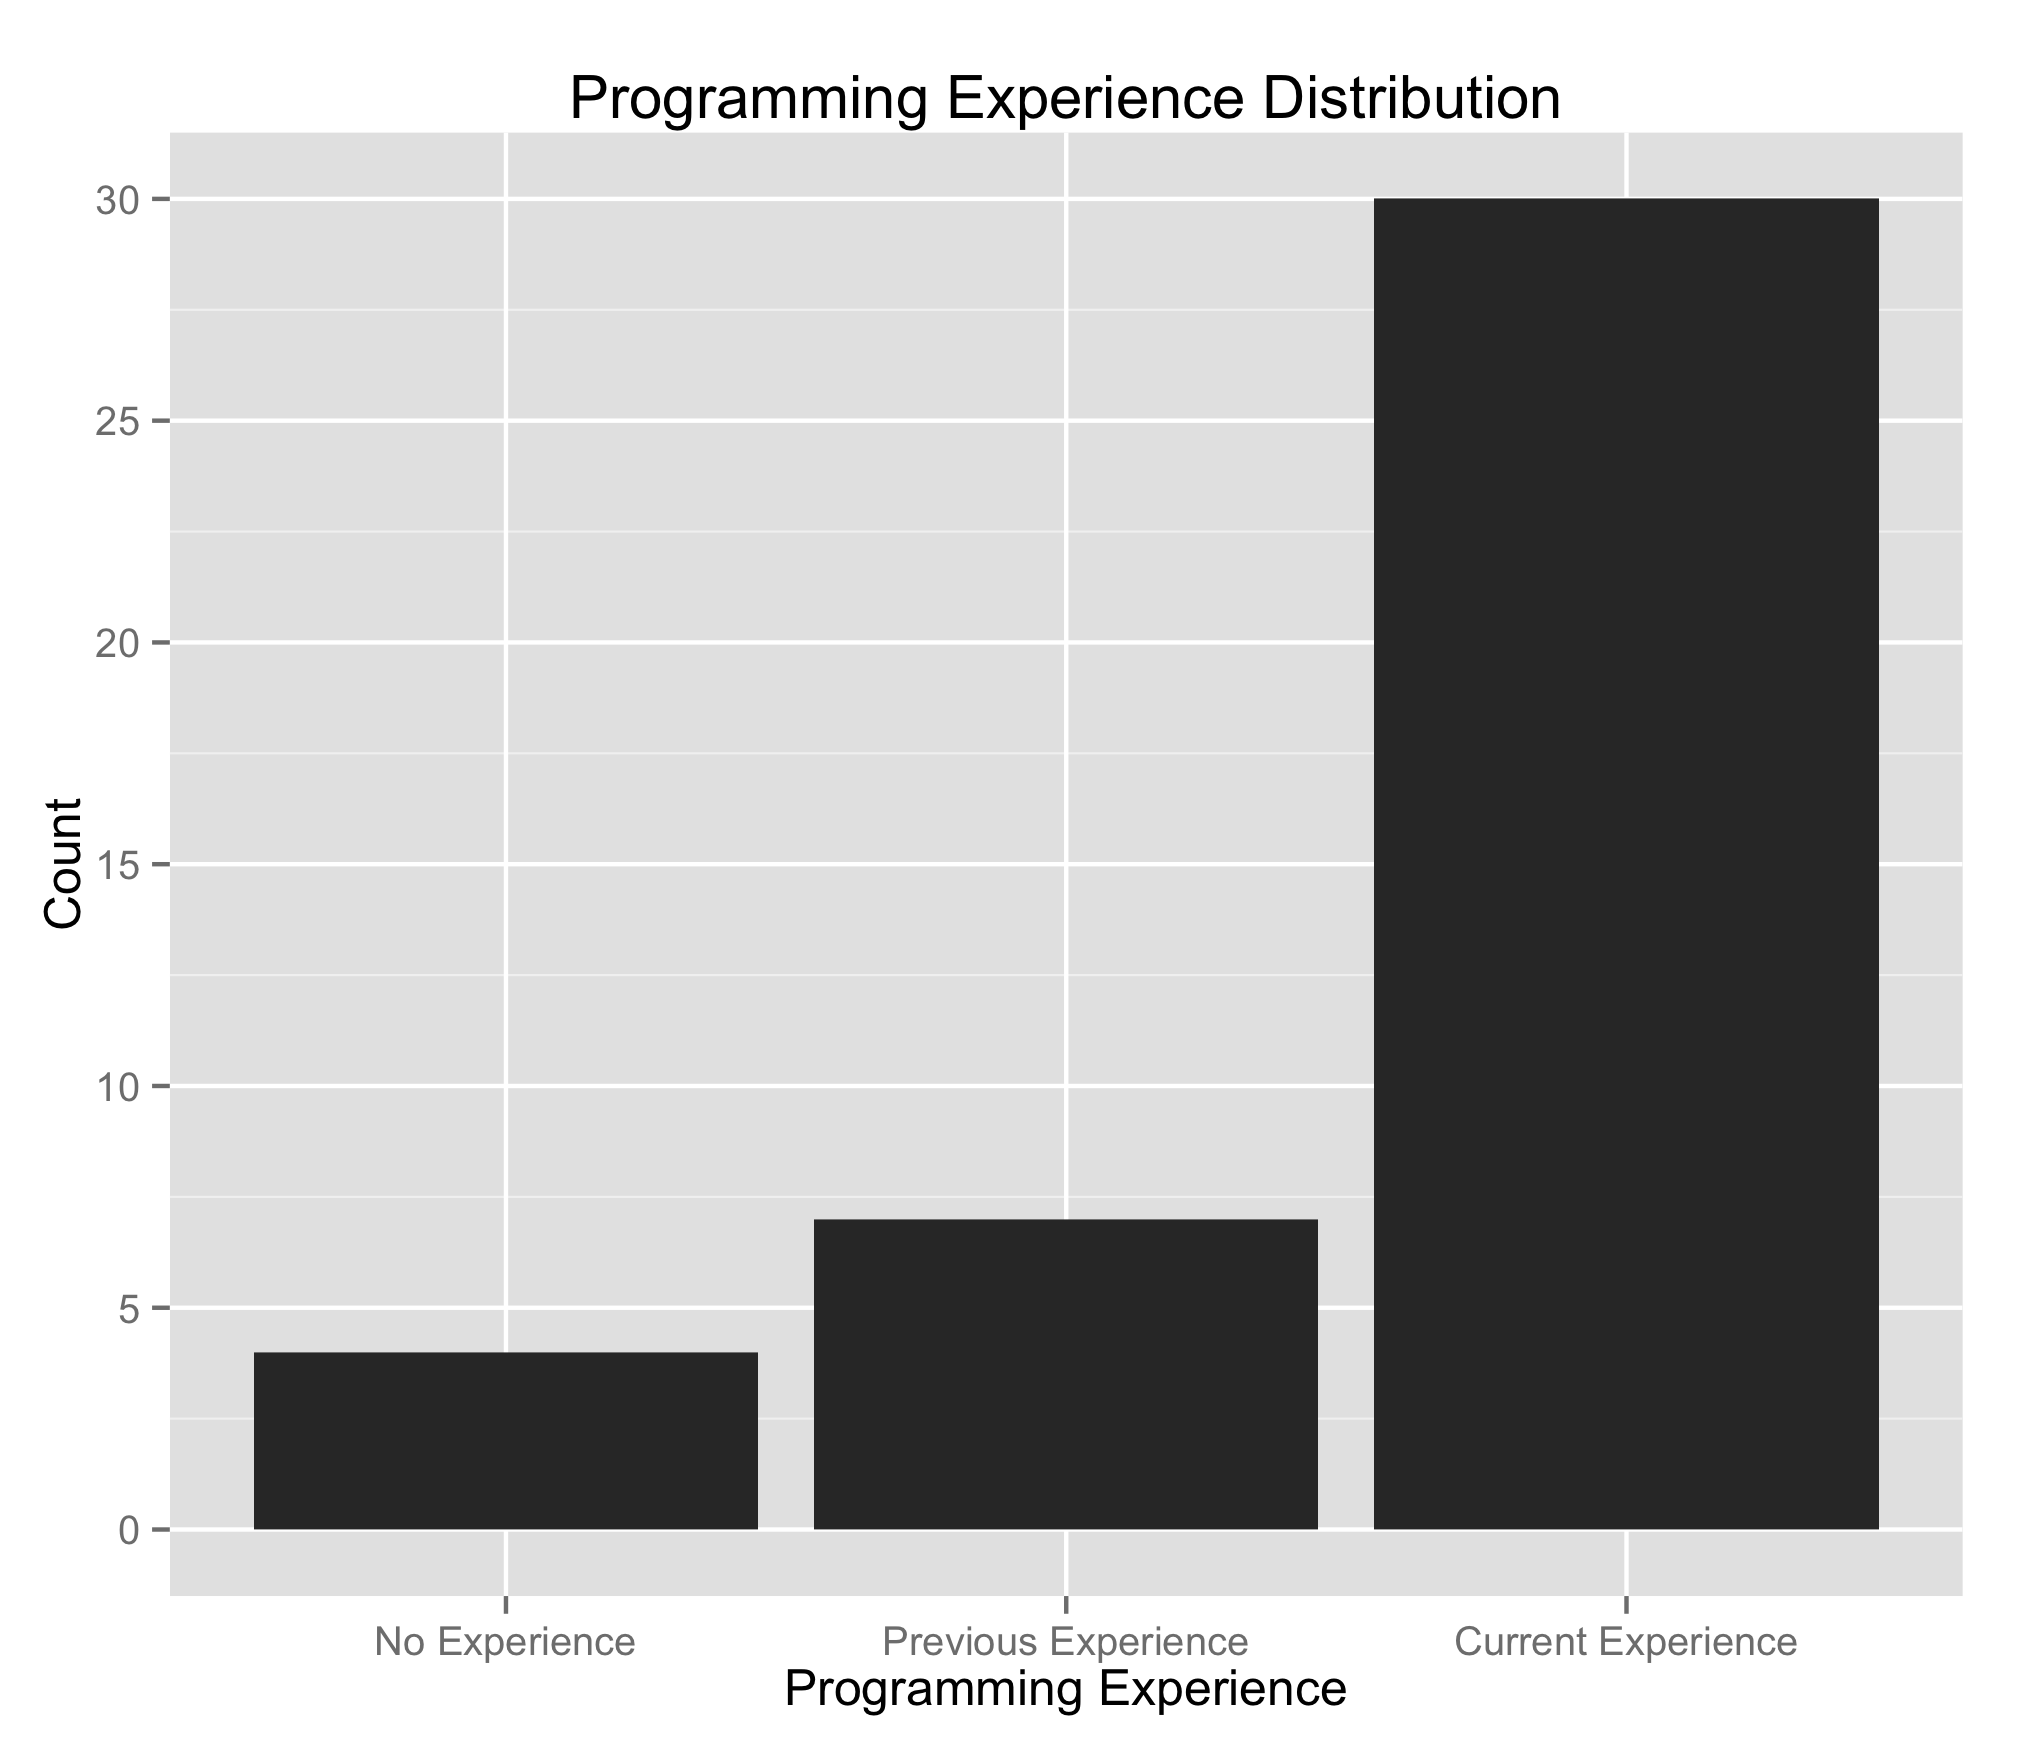
\includegraphics[width=1.0\linewidth]{graphs/programming.png}
    \caption{Programming Experience Distribution}
    \label{programmingdistribution}
\end{subfigure}%
\begin{subfigure}{.5\textwidth}
    \centering
    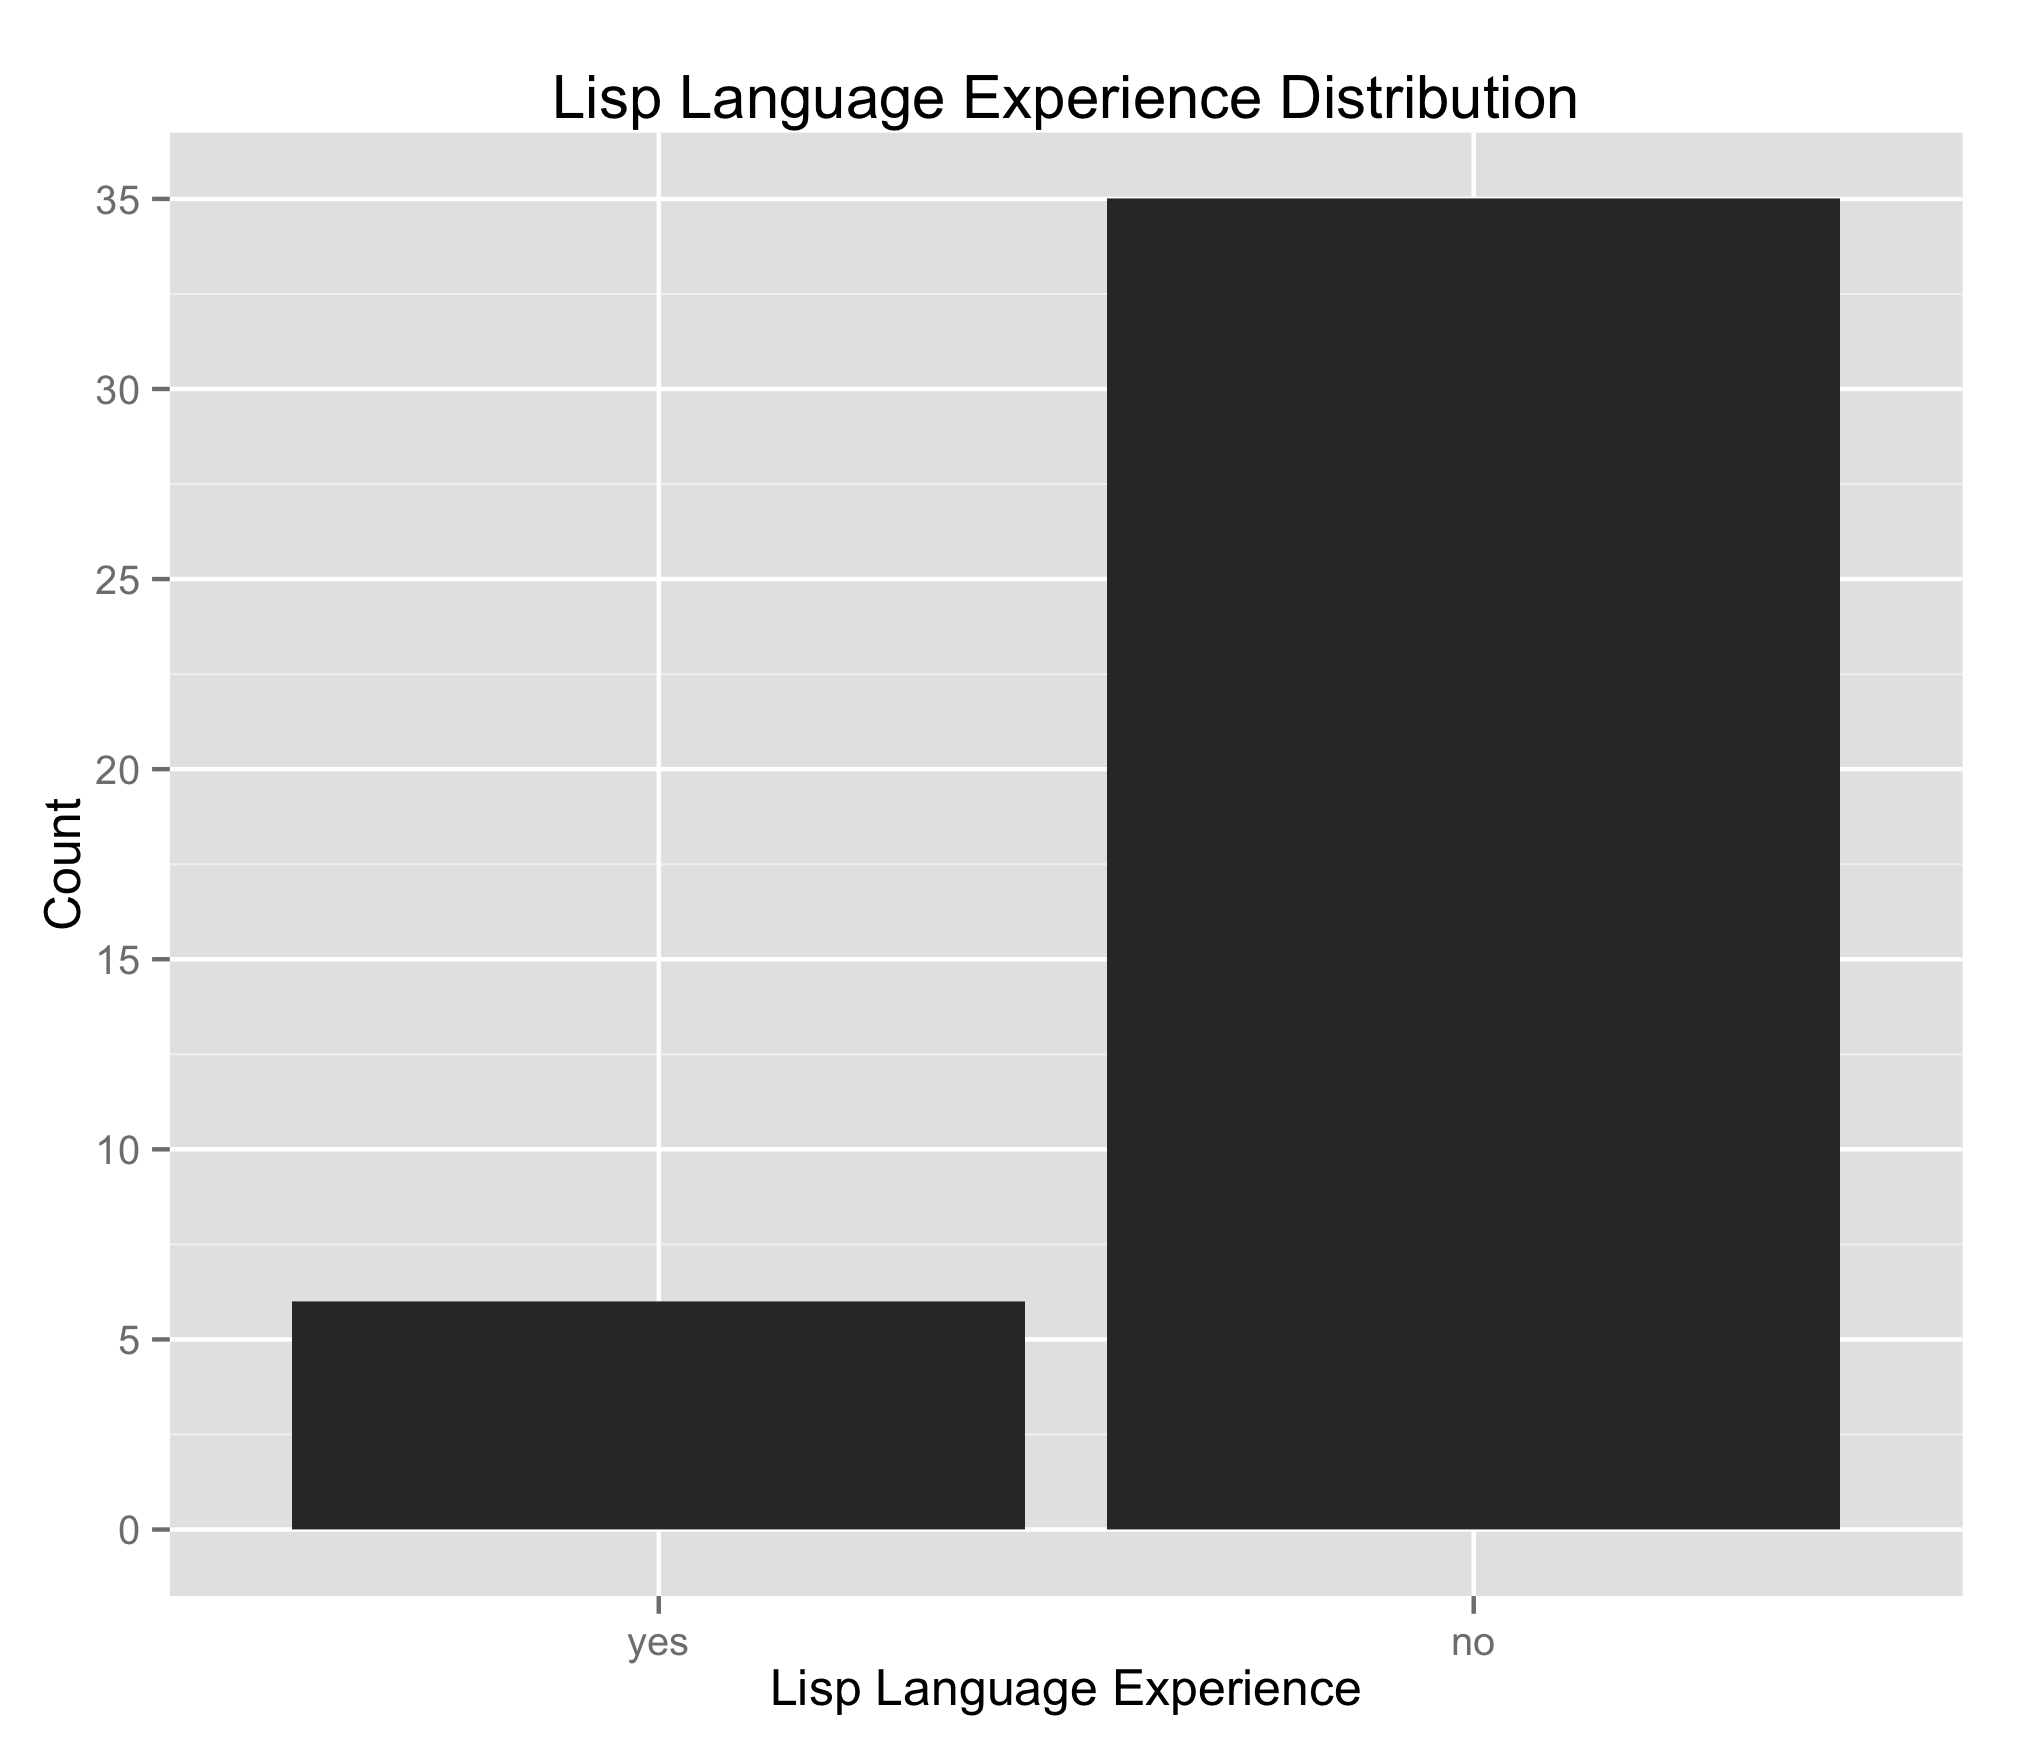
\includegraphics[width=1.0\linewidth]{graphs/lisp.png}
    \caption{Lisp Experience Distribution}
    \label{lispdistribution}
\end{subfigure}
\caption{Programming Demographics}
\end{figure}


\begin{figure}[t]
\centering
\begin{subfigure}{.5\textwidth}
    \centering
    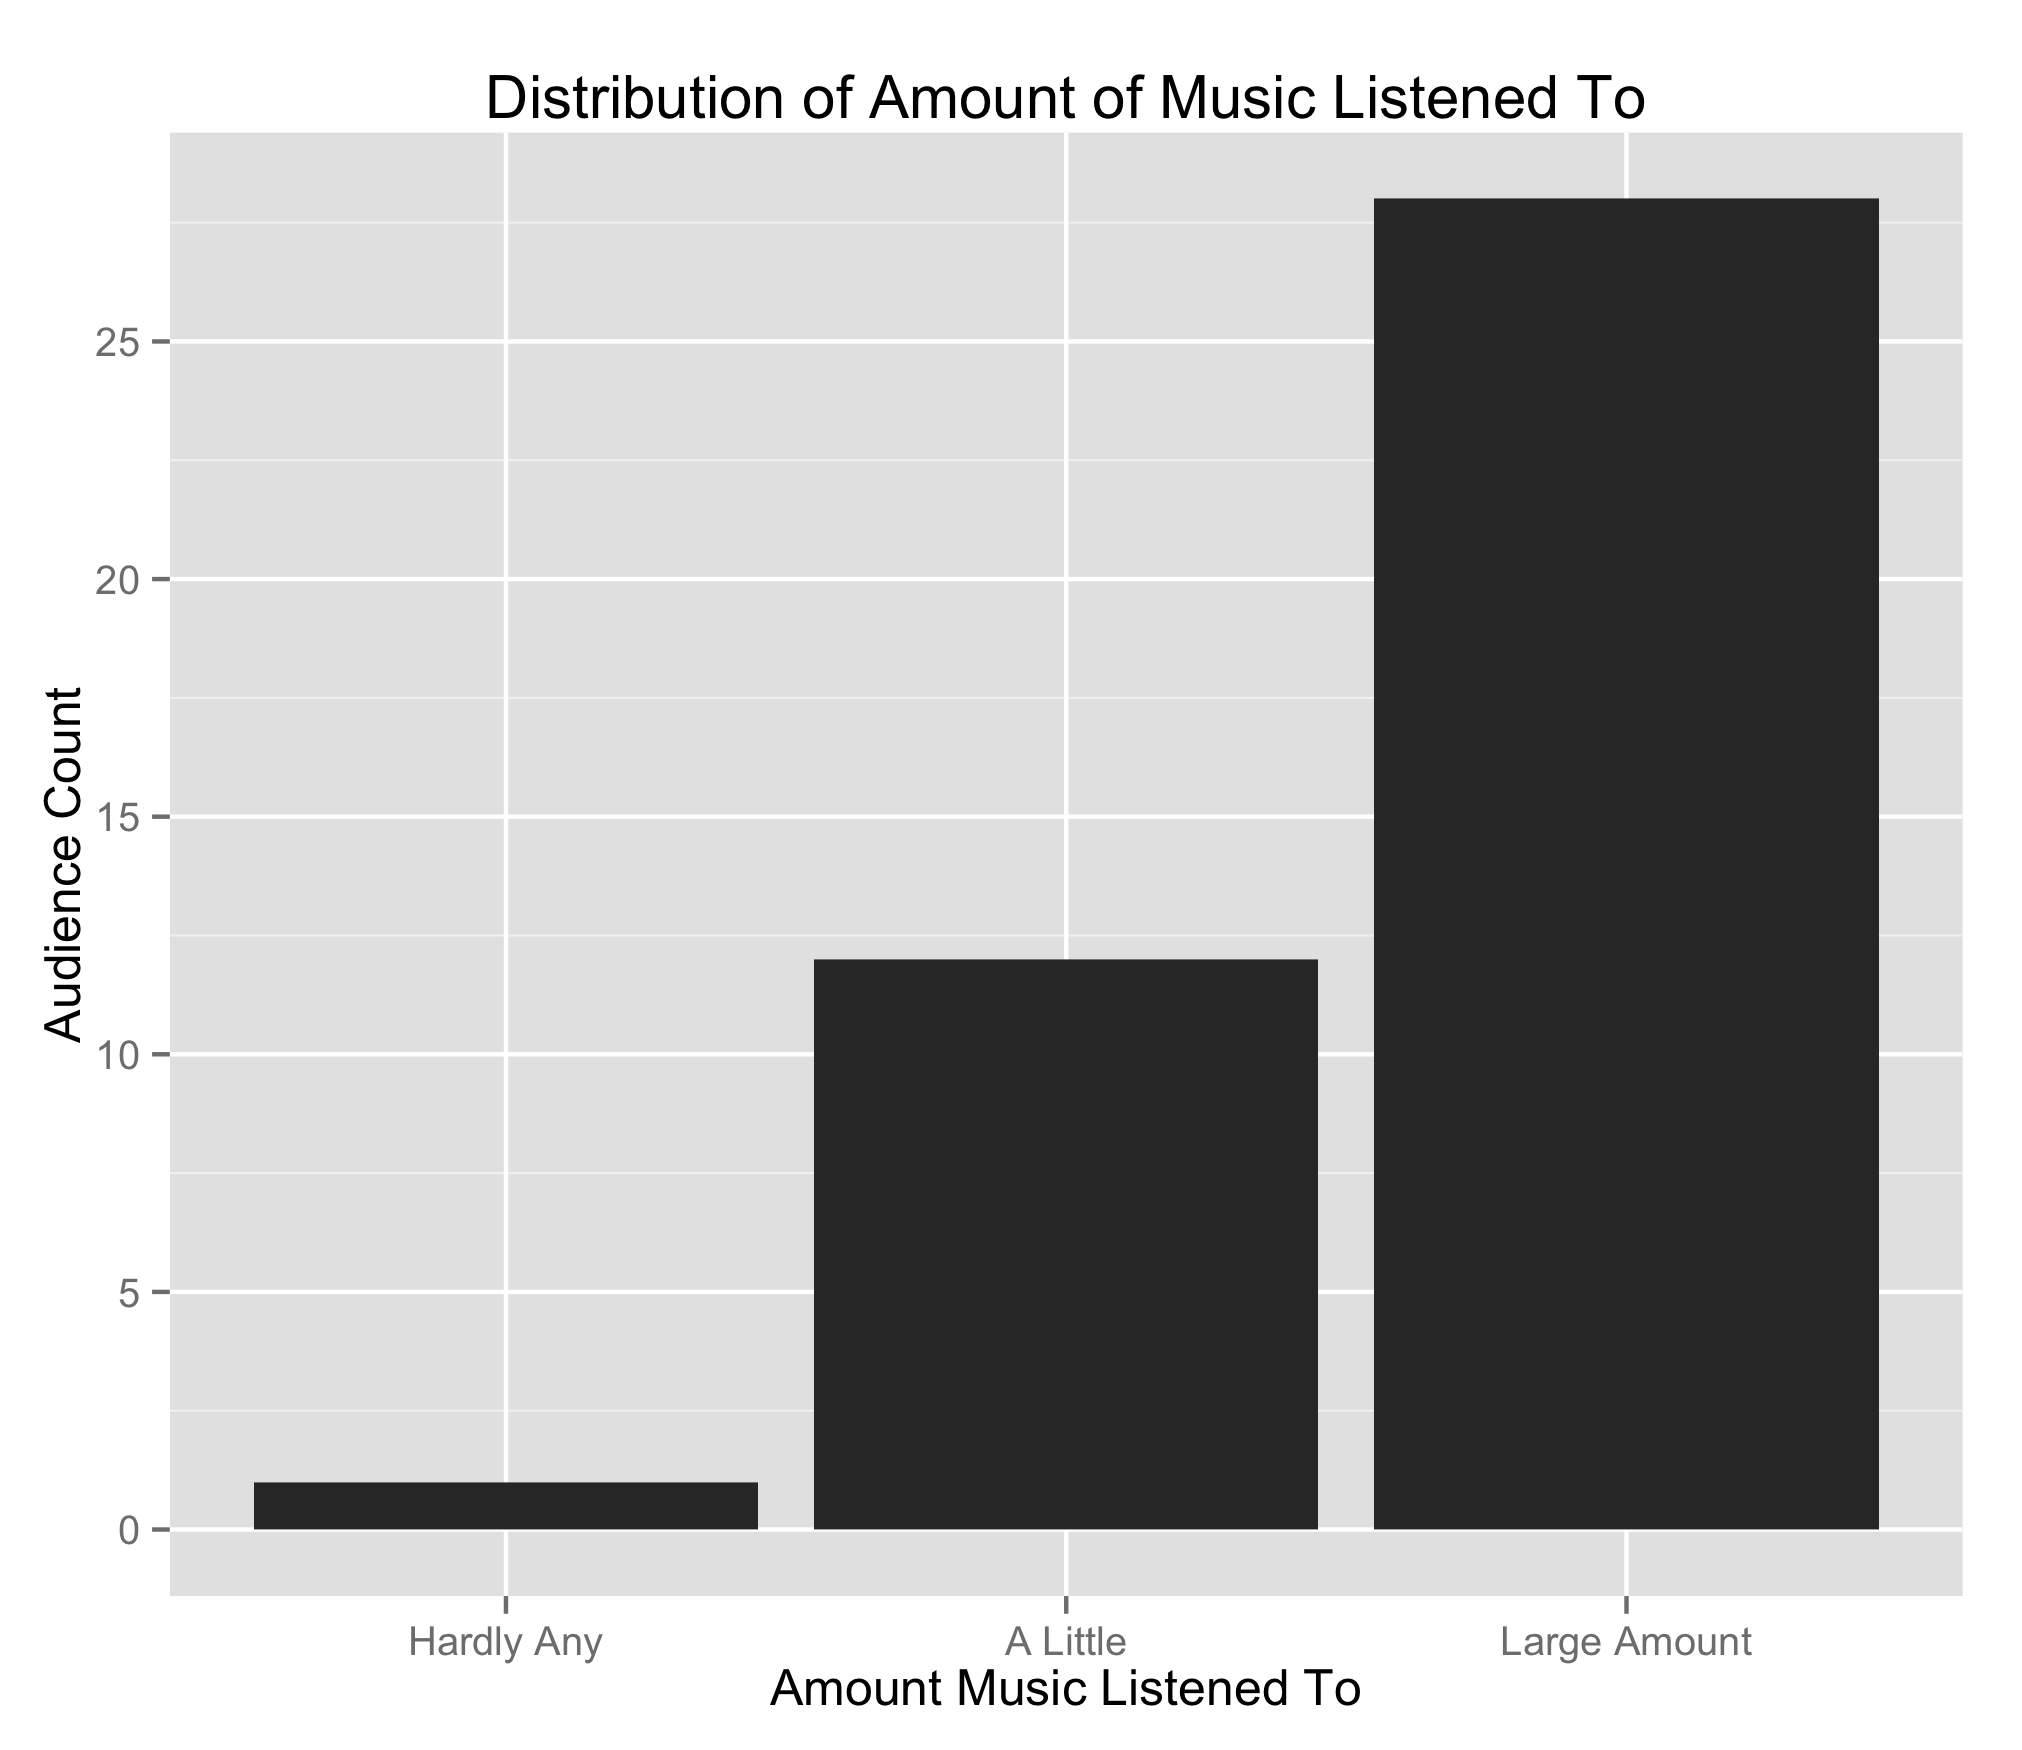
\includegraphics[width=1.0\linewidth]{graphs/music.png}
    \caption{Listen to Music Regularity Distribution}
    \label{musicdistribution}
\end{subfigure}%
\begin{subfigure}{.5\textwidth}
    \centering
    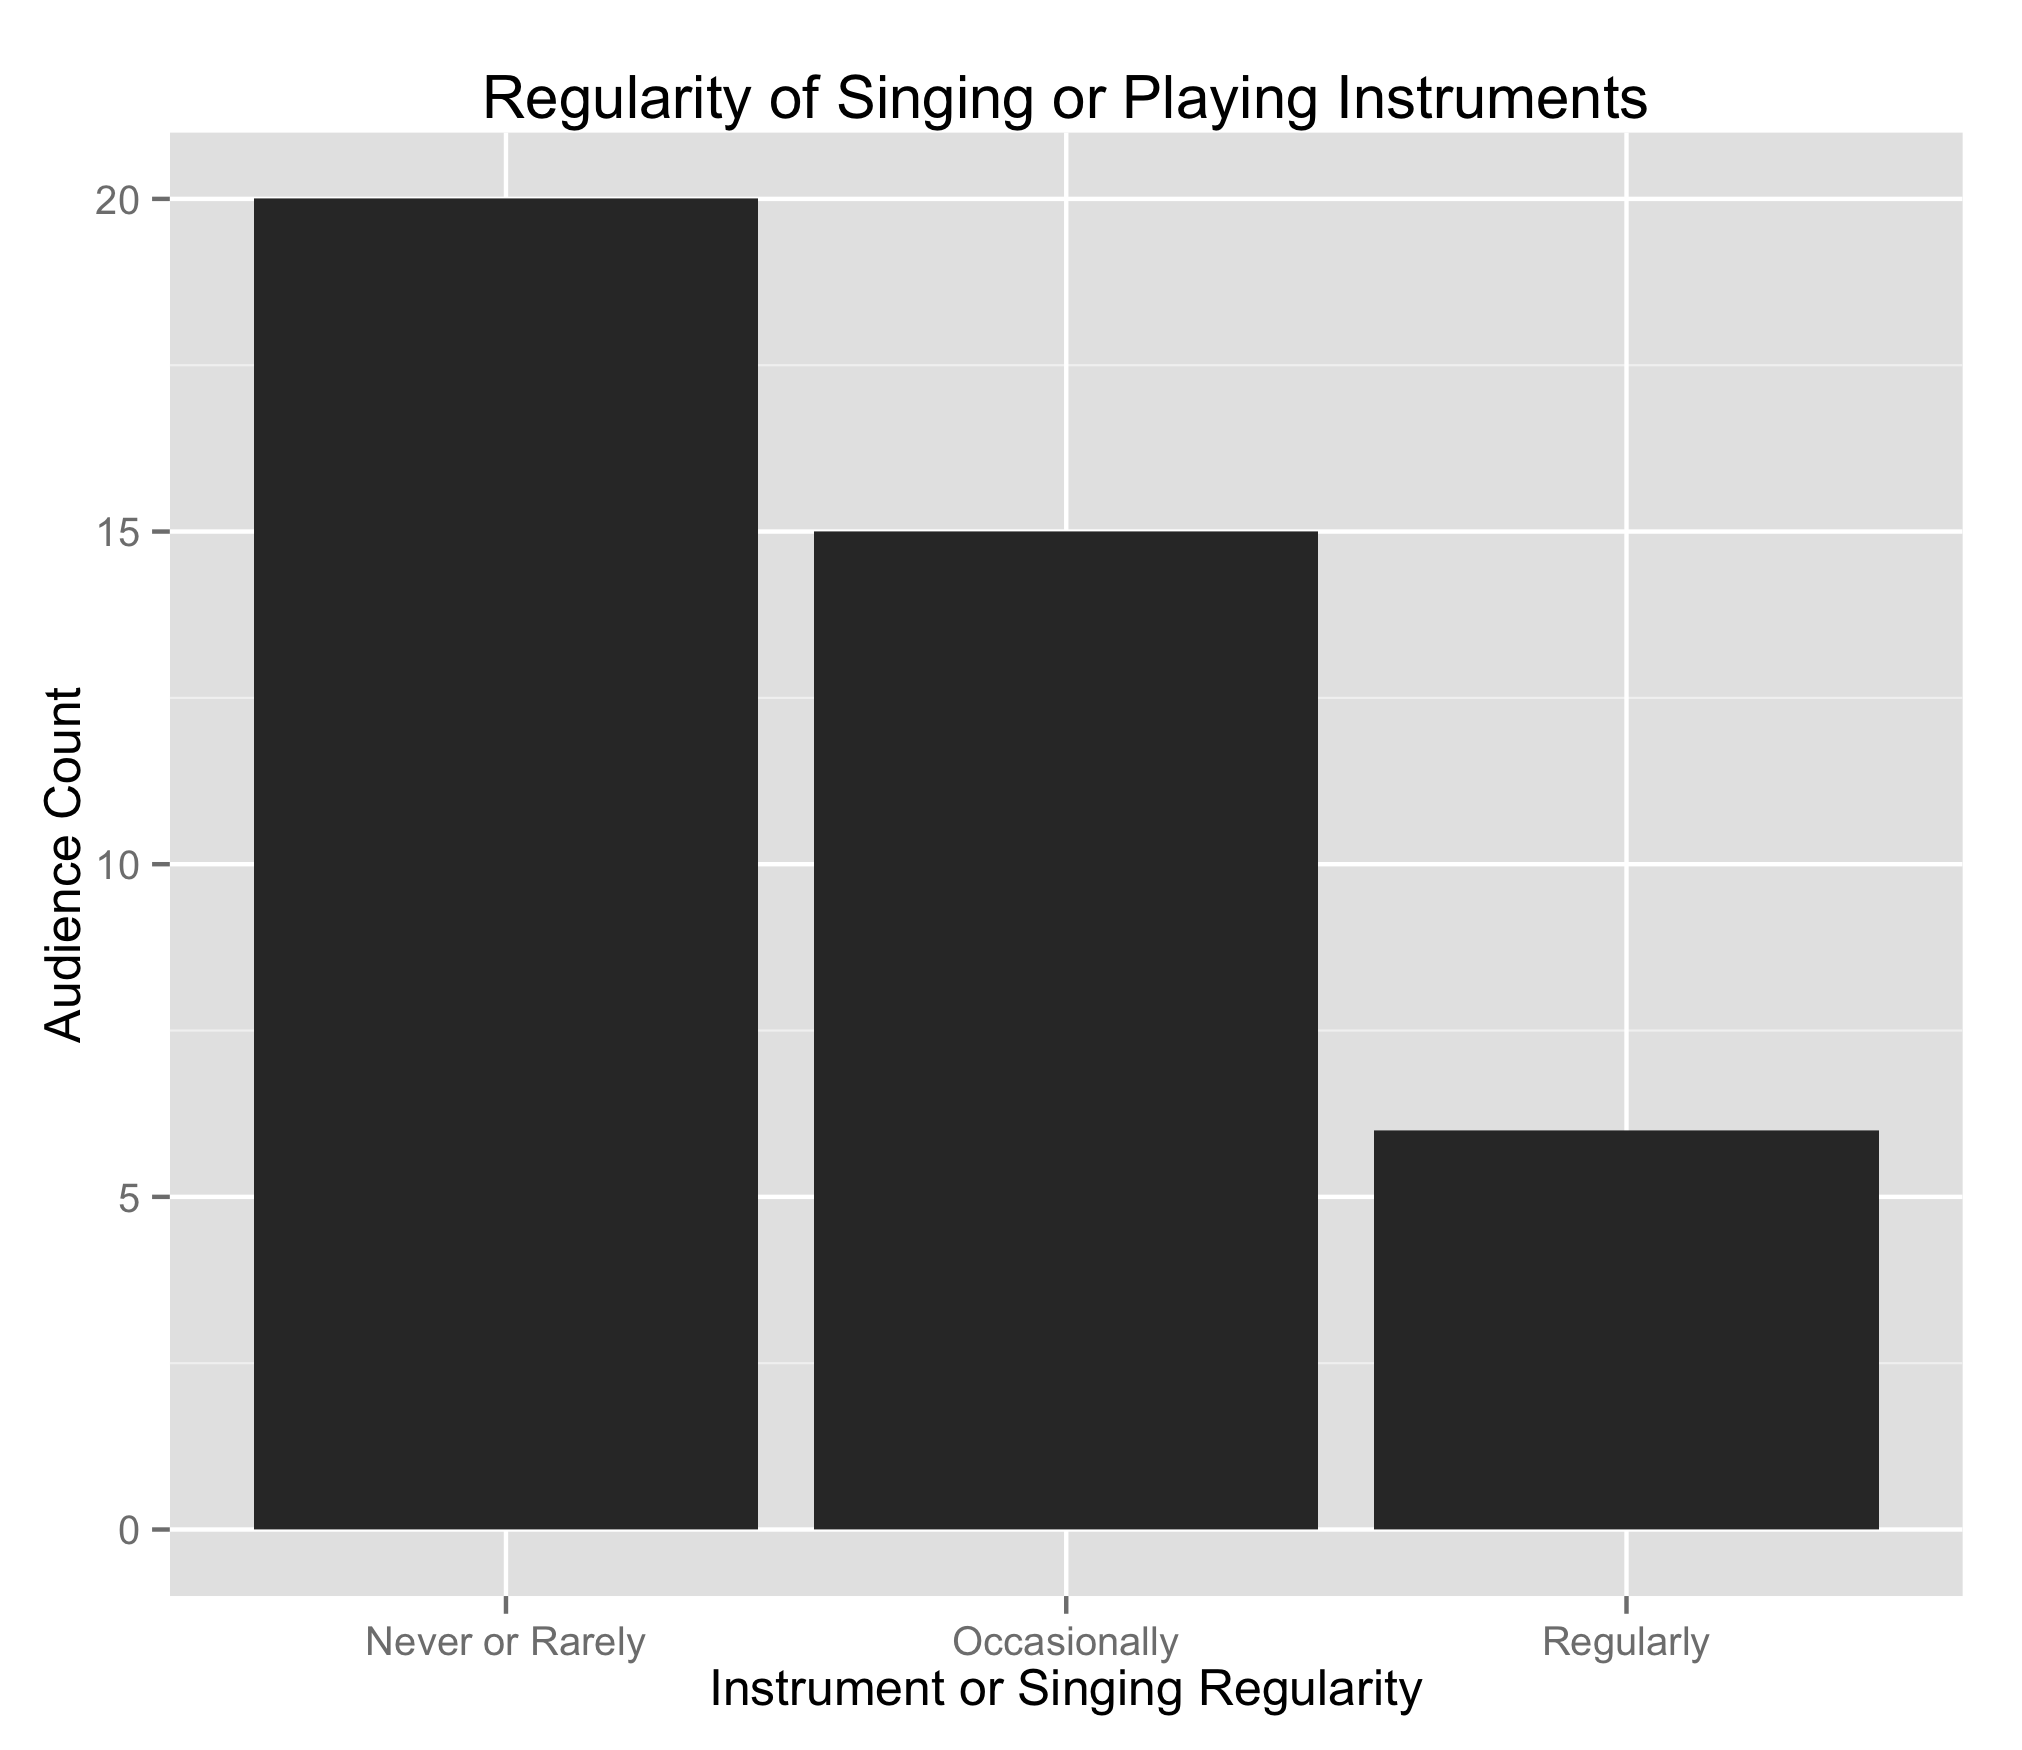
\includegraphics[width=1.0\linewidth]{graphs/instrument-regularity.png}
    \caption{Playing Instrument or Singing Regularity Distribution}
    \label{instrumentdistribution}
\end{subfigure}
\caption{Musical Demographics}
\end{figure}

\newpage
\section*{Appendix B - Survey}

\subsection*{Part A}

Age?\\
18-22\\
23-27\\
28-32\\
33-37\\
38-42\\
43-52\\
53-62\\
63+\\

Gender?   \underline{\hspace{3cm}}\\

How many live coding performances have you been to?\\
This is my first one\\
I have been to one or two\\
More than two. Please indicate the approximate number:   \underline{\hspace{3cm}}\\

How much music do you regularly listen to?\\
Hardly any\\
A little\\
A large amount\\

Do you play an instrument or sing?\\
No - I would not consider myself a musician or singer\\
Occasionally\\
Yes - I play or sing regularly\\

How much experience do you have with programming?\\
No experience\\
Some experience\\
I currently program for my study/hobby/work\\

Do you have much experience with the Lisp family of programming languages? (e.g. Scheme, Lisp, Clojure, Racket)\\
Yes\\
No\\
I don’t know what you’re talking about\\

\subsection*{Part B and C (repeated for the two performances)}

How would you rate your levels of enjoyment during the beginning, middle and end phases of this performance?\\
Circle one alternative for each phase - interpret “beginning”, “middle” and “end” as you wish:\\

Beginning: Low Medium High\\

Middle: Low Medium High\\

End: Low Medium High\\

Did the projected visualisations help with your enjoyment of the code?\\
Yes\\
No\\
No opinion\\

How would you rate your understanding of what the code was doing during each phase? Circle one alternative for each phase - interpret “beginning”, “middle” and “end” as you wish:\\

Beginning: Low Medium High\\

Middle: Low Medium High\\

End: Low Medium High\\

Did the projected visualisations help with your understanding of the code?\\
Yes\\
No\\
No opinion\\

This was a live performance! Did the projected code and visualisations help communicate the feeling that the performance was live? If so, how?\\

\hrule \bigskip \hrule \bigskip \hrule \bigskip \hrule \bigskip \hrule

\subsection*{Part D}

Do you have any suggestions for how the visualisations for either performance might be improved? (Continue answer on the back of this sheet if you wish)\\

\hrule \bigskip \hrule \bigskip \hrule \bigskip \hrule \bigskip \hrule \bigskip

\newpage
\section*{Appendix C - Visualisations}

\begin{figure}[H]
\centering
\begin{subfigure}{.5\textwidth}
    \centering
    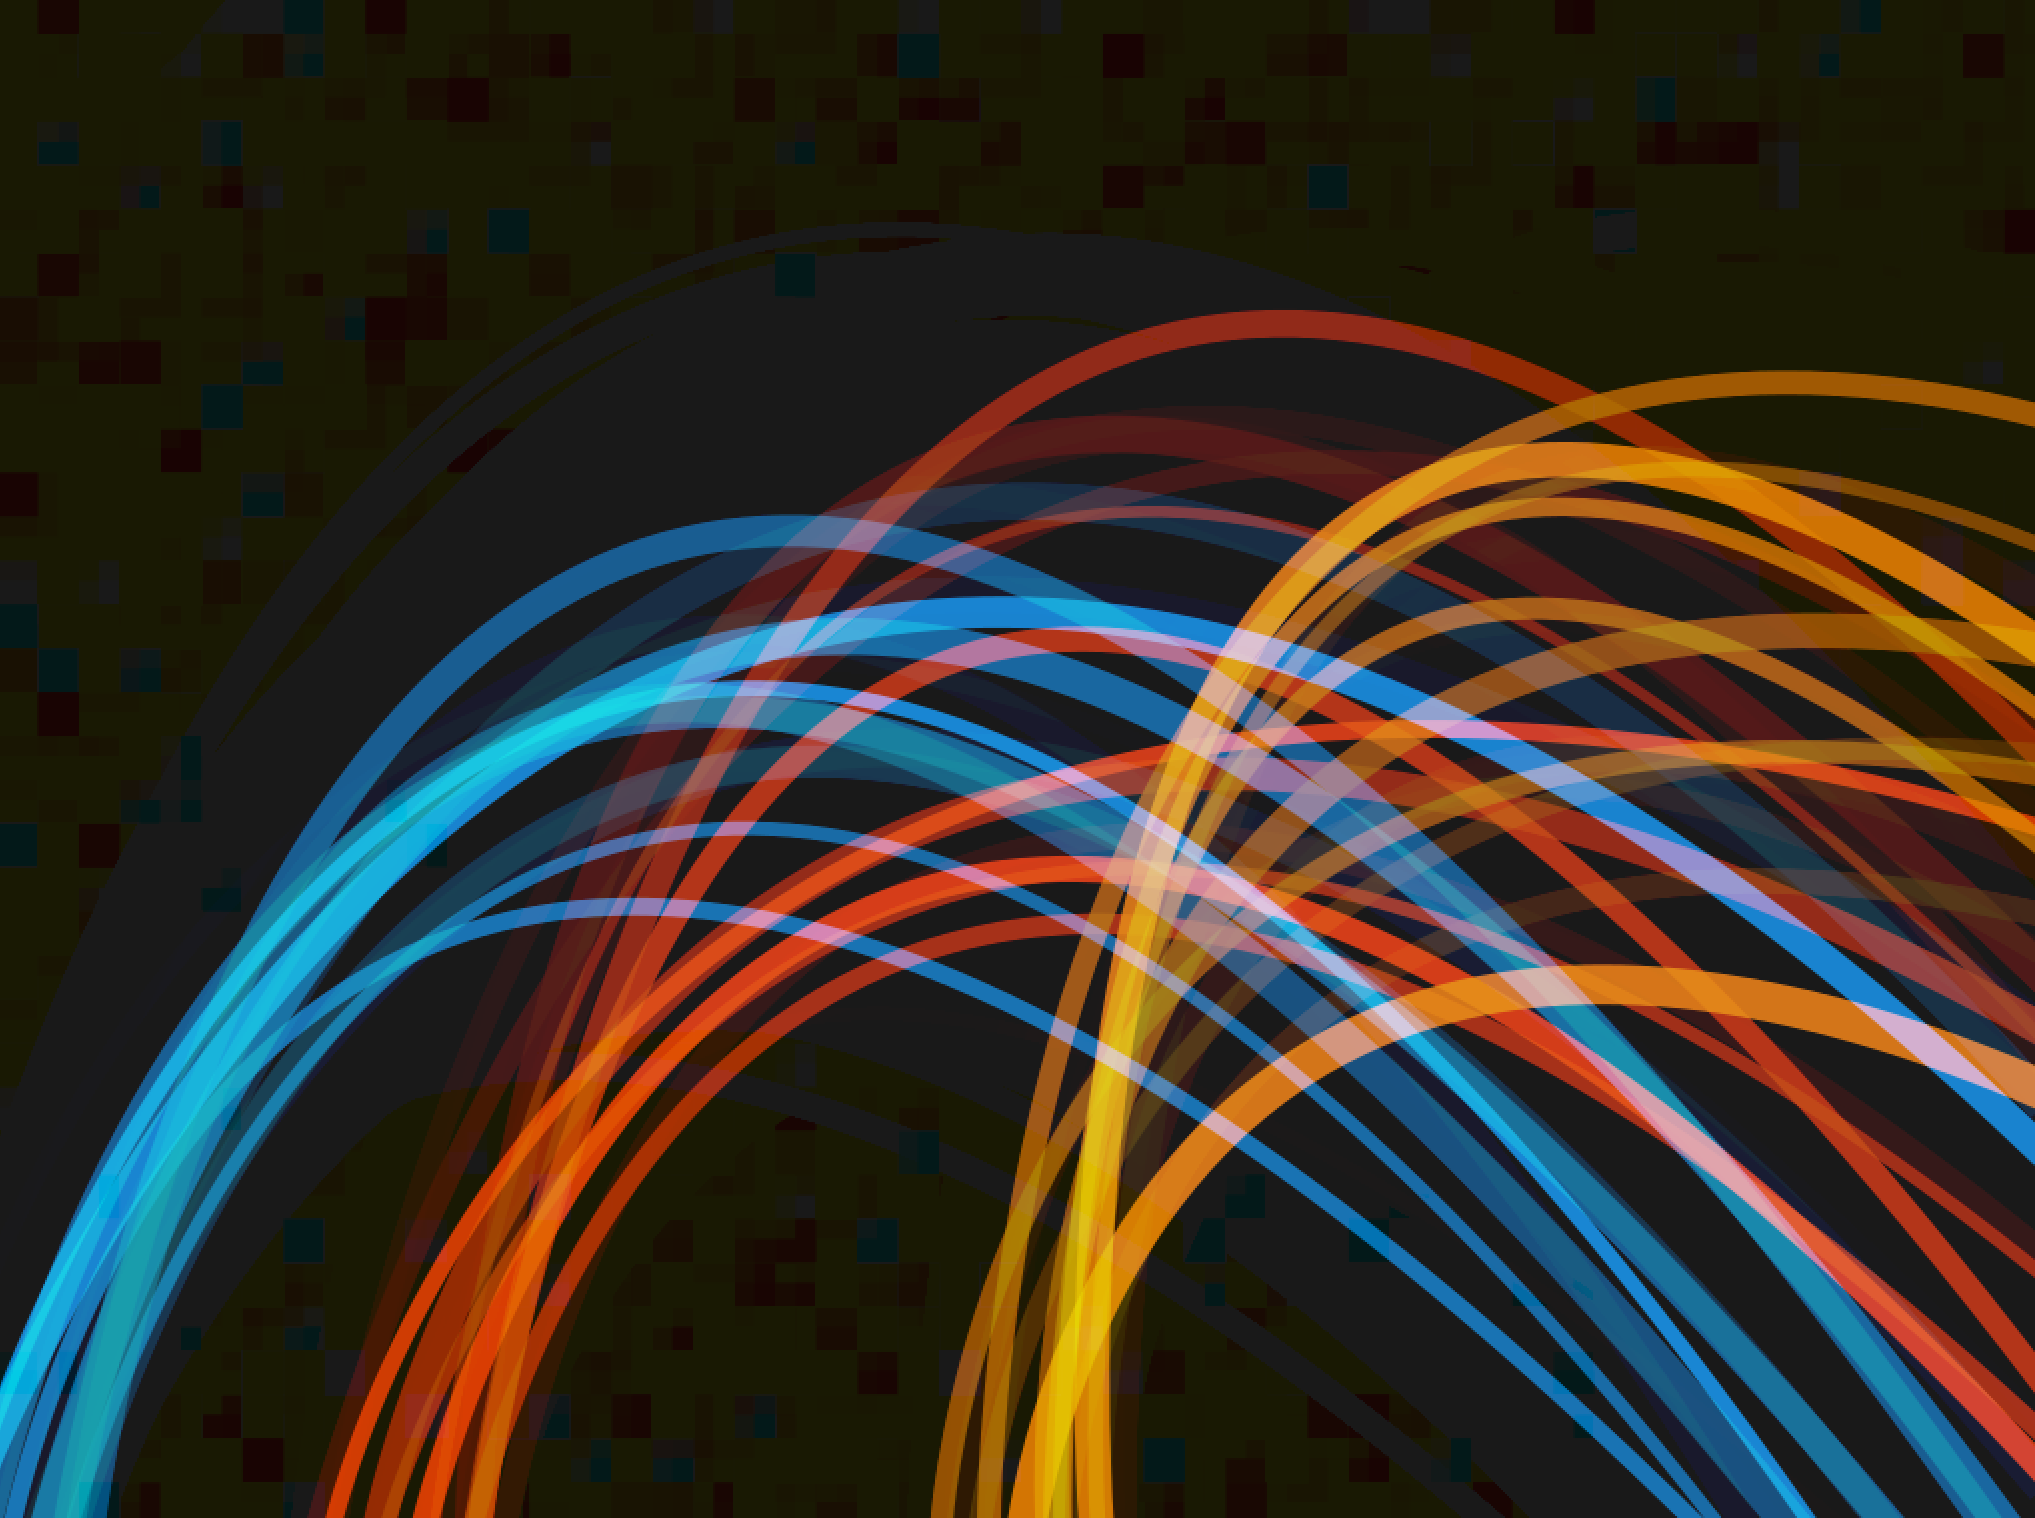
\includegraphics[width=0.9\linewidth]{visualisations/aesthetic-vis.png}
    \caption{Aesthetic Visualisation}
    \label{avis}
\end{subfigure}%
\begin{subfigure}{.5\textwidth}
    \centering
    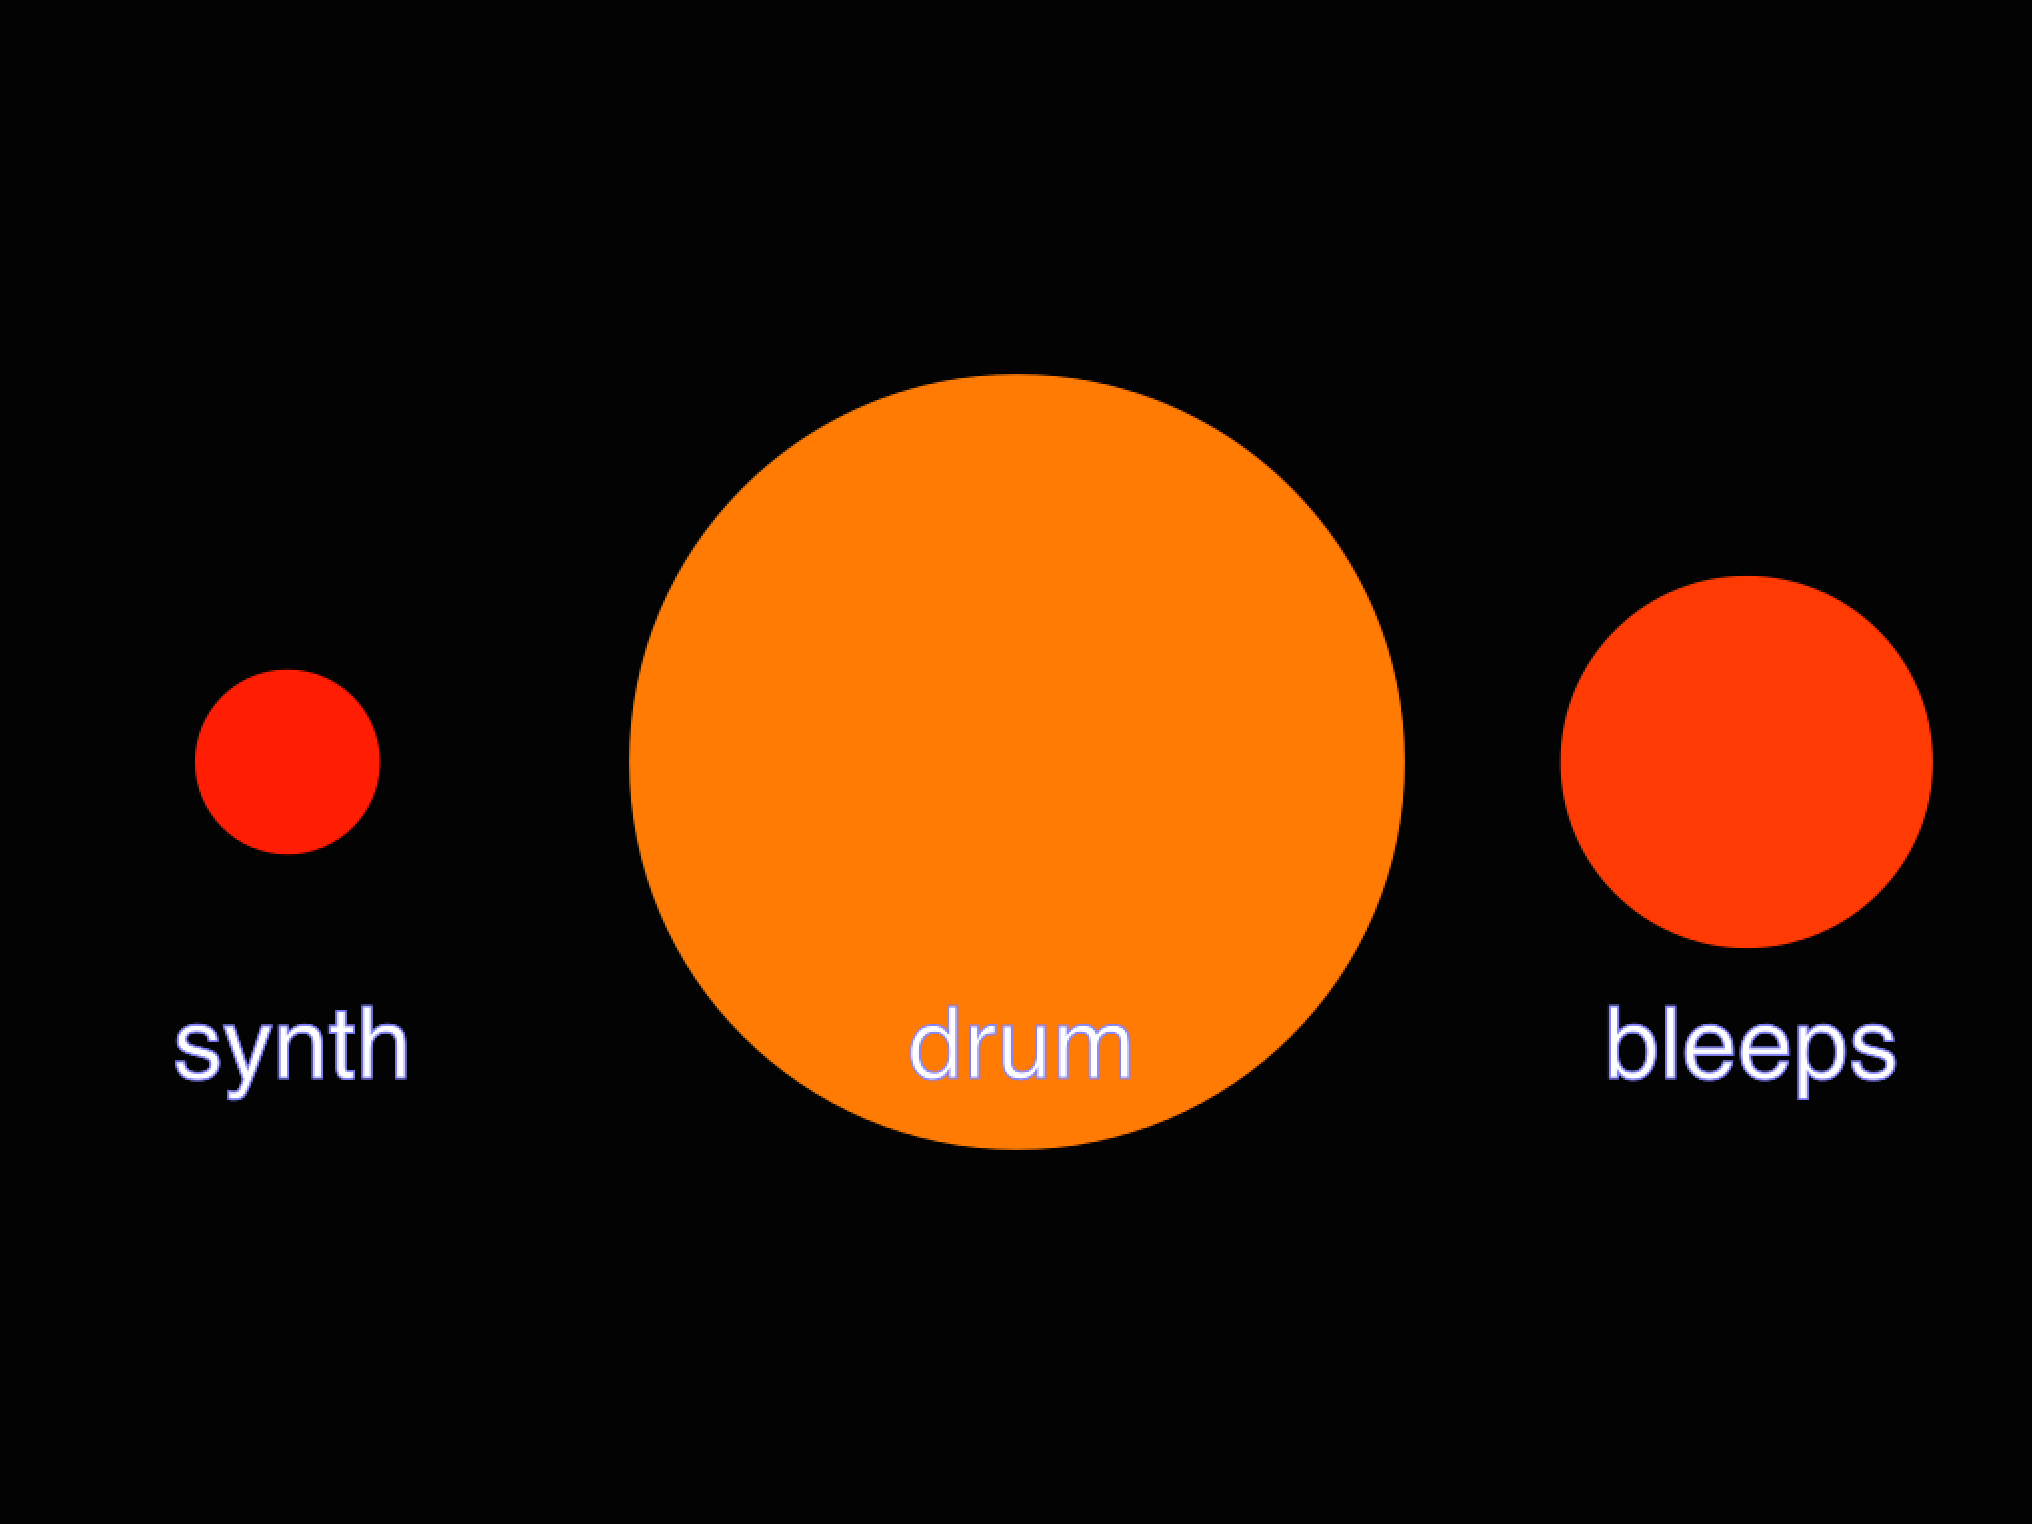
\includegraphics[width=0.9\linewidth]{visualisations/didactic-vis.png}
    \caption{Didactic Visualisation}
    \label{dvis}
\end{subfigure}
\caption{Visualisation Examples}
\end{figure}

\section*{Appendix D - Interview Transcript}

\subsection*{Aesthetic Visualisation}

Ben: So the first little synth thing in this I knew pretty much exactly what I wanted to do. I was going to do random pitches at 16th notes. I think I probably did this synth thing exactly the same in other performances.\\

Arrian: Is this a common technique you use?\\

B: Yeah, well. This was not even prepared specifically for this performance but I've done stuff like this in the past. This is a pretty common trick I use for getting up and running early.\\

I think the bass is playing at this point but I can't hear on these speakers.\\

A: How much planning went into this performance?\\

B: This performance was pretty safe. It was pretty simple and pretty preplanned. What I would say is that the form of all of the instruments are pretty standard for my live coding.\\

So for the bass to go through a list of pitches like that... I do that alot.\\

For the drums I play with some sort of modulation of the sample slot, of the kit... I do that alot.\\

I probably choose slightly different parameters each time through but, yeah, none of these things are really adventurous by the standards of my live coding.\\

A: Why is that?\\

B: Honestly, the main reason is that these things work well and I've tried other algorithms and they don't sound as good as these simpler algorithmic structures with judicious choice of parameters.\\

Though I feel that as an artist sure, as a programmer this is not so interesting because the algorithms are pretty safe.\\

There are a lot of people in computer music today that use fancy algorithms, they use cellular automata, they use generative algorithms but I think it works better if you use... I've had more artistic success using these simple algorithms and then just using my musical experience and intelligence to select good parameters...\\

A: Did you plan the performance around the visuals?\\

B: To be honest, I think in the second piece I tried to limit the callback rate because I knew that some of the visuals in the didactic setup worked better with a longer callback rate.\\

A: Do you think the visualisations held you back?\\

B: No, it certainly didn't hold me back. In some ways it is nice to have constraints.\\

I'm now going up an octave. It gives it a harder edge...\\

It is interesting that I'm very conscious of the hypermeter. I'm just grooving along and it just makes sense to evaluate in time.\\

A: Did you find this visualisation distracting?\\

B: Ah, no. In general I'm just so focussed on the code.\\

This little bit is adventurous. This drum bit I didn't know exactly what samples were in those slots. Before I was just guessing some numbers and picking numbers I thought might be good.\\

This bit is certainly more intense. This is more european house. I don't actually know if it is european house but I'm sure there is some name for this genre.\\

This end bit is a bit new. I hadn't planned to end it like that.\\

A: Did it occur by chance?\\

B: Not so much by chance. I got to the end and wasn't really sure how I would finish this. This is true making it up.\\

A: Were you happy with the performance?\\

B: Yeah.\\

I'm actually going diatonically out of the scale I was using for the whole piece.\\

Yeah, I hadn't planned to finish like that but... yeah, yeah, I'm reasonably happy with that.\\

B: I think in terms of the surprising stuff. There were no surprises when I started or added each new instrument. I knew pretty much exactly what I was going to do. I might not have had the exact parameters in mind. I would have put maybe a 60 instead of a 70. Even when I didn't have an exact number in mind I would have had an approximate number in mind... loud vs soft.\\

Once stuff is going then I think all bets are off and I at least don't really think through what I'm going to do after that. Generally I'll go back and start messing with stuff. In that case I went back and messed with the synth.\\

I did a bit of interesting stuff with the drums. I went from a more groovy and pretty standard drum beat to a heightened beat which definitely changed the mood of the piece.\\

I'm not unhappy with that. I'd probably do something different next time just because you do something different every time but that was one of the things that surprised me.\\

In general I was pretty happy with it. I think it is a good sound palette. The drums grooved pretty well which is an important thing. The bass line was pretty cool, though I couldn't hear it in that recording.\\

A: In terms of the visualisations, do you think they added anything to the piece?\\

B: I think they added something. I think they are just ambience. It is definitely cool to have that stuff going on that is a little visually interesting but I wasn't paying attention to them even then. I definitely wasn't paying attention to them on the day. In fact I tuned them out as best I can because I am just trying to focus on the code.\\

Like I was saying before there were times where it was hard to see the code underneath the visualisations.\\

A: Was this during the aesthetic or didactic performance?\\

B: I think it was more the didactic and I think it was the text in the didactic ones and not in the aesthetic.\\

I definitely like the visuals. They definitely add something and they don't take anything away even though I wasn't paying attention to them. I still see the text as the main thing but the visuals are gravy and that was nice gravy.\\

A: The audience was reasonably computer literature. Do you think they would have preferred to focus on the code, the music or the visuals?\\

B: That's a good question. I don't know. I'm really curious.\\

Focus is a funny thing. You rarely explicitly go ``alright, I'm going to focus on blah and focus on blah''. I think you drift. Probably at different points they were paying attention to each.\\

I think I'm a bad judge of what people pay attention to because I pay attention to completely different stuff when I watch it. What I pay attention is probably completely unhelpful in terms of an indicator for what even a computer literate audience member would be paying attention to.\\

\subsection*{Didactic Visualisation}

Ben: Now this one starts at a slower tempo. Half the speed... 60bpm vs 120bpm.\\

Arrian: Was this due to the nature of the visualisation?\\

B: No, that was just to be different. They both work fine with the visualisations. In fact the visualisation pretty much work with whatever tempo.\\

So this one is a slower starting one. I still get it going fairly quickly.\\

A: Did the visualisations get in the way here?\\

B: It wasn't too bad because it's not over the top of where I was trying to work.\\

This is one of the things that I did have the visuals in mind when I put together this thing. Initially you have the fast spinning visuals. I knew that I was going to slow this one down and go for two bars of eight beat long sustained chords. I knew that that would look cool as a slowly rotating thing.\\

In fact I stuffed it up there. It wasn't so much a typo as I did a tricky thing where I tried to have a couple of overlapping temporal recursions and filter out only the fast one keeping the slow one going. But that relies on changing the code once you've got it to the state you want.\\

I think in general with these parameters I was just messing around. I knew the general form.\\

I've got a couple of polyrhythms. I really like this bit. I think it works well.\\

A: Despite the timing issue with the visualisations?\\

B: Timing is off by half. We knew that was a problem. I still think it works pretty well. I think this one has real potential but it is disappointing that they didn't sync up.\\

This one is just grooving. I quite like the beat in this one.\\

A: Did the visuals affect your ability to see here?\\

B: I can't remember to be honest. It wasn't a big problem to be honest. It probably only happened once through all four pieces.\\

A: Were you tuning out these visuals during the performance?\\

B: Even when I'm watching it I'm tuning out the visuals but definitely during the performance.\\

I don't think this was planned. It is a fairly standard part of my live coding toolbox. I'm just changing the pitch. So it's to do with the bass. Quick ones and then long ones.\\

Then I changed the offset of the chords and the chords would come in staggered. I don't know how well this one worked in the end. I like bits of it but...\\

This one I think the stuff that is kind of up beat and is really groovy is easier to do than this.\\

This bit was disappointing. I had a cool ending in mind and the I stuffed it up here. I forgot to put the tick symbol.\\

A: Did you manage to pull off the cool ending in the second performance?\\

B: No, I tried to do the same thing and stuffed it up in the exact same way. That was interesting and frustrating. I had a cool ending that I just thought of that day where I was going to do some harmonic organ-y stuff, take it through the circle of fifths and do an interesting chord progression but really kind of draw one out for a slow finish. I just forgot to quote that symbol when I went from the minor to the major.\\

If I had other instruments covering me I could of started it again but since everything had died if I started it again it would have been really obvious so I decided in the moment that that is where I would finish it whereas I had one more minute planned. I started to go down a path where I had a minute more of material to finish it off but then just dogged it. Frustratingly I did not quite the same mistake but a similar sort of mistake in the second one. It's kind of really rare... obviously I make typos but I don't tend to make them in that way.\\

A: Was there some reason for the mistakes?\\

B: Not really.\\

A: Chance?\\

B: Yeah, just chance. Just life.\\

A: Was the main goal of this performance to entertain the audience... beyond the research?\\

B: Yeah, I think so. I always want the people to enjoy themselves. I tried to keep them pretty short. I think every little set was under ten minutes. If you're going to do a live coding set longer than ten minutes it needs to be bloody good. So in general I try to stay under ten minutes.\\

It's interesting, some of my earlier videos are longer than ten minutes and I watch them now and I think `this drags on'. I'm much better at it now and I'm much better at making things happen quickly. I'm especially better at getting stuff up and running, partially because I'm an emacs guru and have all the snippet magic to make that happen but also you just learn the little extempore tricks and the general tricks for getting things up and running.\\

For example in the aesthetic set, there was probably stuff going after only 10 seconds. For this one there was probably stuff up before 30 seconds. I reckon you've got to get something up before 30 seconds.\\

A: Was boredom getting to you?\\

B: Not really. Certainly not in a big way. By the fourth I was like ``I'm done, this has been a lot of live coding, I'm sort of out of ideas".\\

It's not even fair to say `out of ideas'. I had that cool idea about how I was going to finish it that I dogged both times. It's just exhausting. It really does take a lot of concentration.\\

I was done at the end and I was pretty happy it was done. I enjoyed it, I had a good time but I was glad it was done.\\

\end{document}